% =====================================================================
% MSc Dissertation (Final Report)
% MSc Computational Finance, King's College London
% Huseyin Sarp Vulas  -  Supervisor: Dr Bart de Keijzer
% Final submission: 6 August 2026
%
% Build figures first:  python scripts/make_figures.py   (writes docs/figures/*.dat)
% Compile:              pdflatex dissertation && pdflatex dissertation
% =====================================================================
\documentclass[11pt,a4paper]{article}

% --- Encoding / fonts (handles s-cedilla, u-umlaut in author name) ----
\usepackage[utf8]{inputenc}
\usepackage[T1]{fontenc}
% Scalable Type1 fonts are required for reliable PDF text extraction (the CM
% bitmap fonts have no Unicode map). Prefer Latin Modern; fall back to Times
% (mathptmx) where lmodern is unavailable (e.g. minimal TeX installations).
\IfFileExists{lmodern.sty}{\usepackage{lmodern}}{\usepackage{mathptmx}}
% Map glyphs (incl. fi/fl/ff ligatures) back to Unicode for copy/paste & search.
\input{glyphtounicode}\pdfgentounicode=1
% Explicit maps for Turkish glyphs in the author/citation names.
\pdfglyphtounicode{scedilla}{015F}\pdfglyphtounicode{Scedilla}{015E}
\pdfglyphtounicode{uni015F}{015F}\pdfglyphtounicode{dotlessi}{0131}
\pdfglyphtounicode{Odieresis}{00D6}\pdfglyphtounicode{odieresis}{00F6}

% --- Layout -----------------------------------------------------------
\usepackage[margin=2.4cm]{geometry}
\IfFileExists{lmodern.sty}{\usepackage{microtype}}{\usepackage[expansion=false]{microtype}}
\setlength{\parskip}{4pt}
\setlength{\parindent}{14pt}
\usepackage{enumitem}

% --- Maths / tables / figures -----------------------------------------
\usepackage{amsmath,amssymb}
\usepackage{booktabs}
\usepackage{array}
\usepackage{multirow}
\usepackage{graphicx}
\usepackage{xcolor}
\usepackage{caption}
\usepackage{subcaption}
\captionsetup{font=small,labelfont=bf}

% --- Plots / diagrams -------------------------------------------------
\usepackage{tikz}
\usepackage{pgfplots}
\pgfplotsset{compat=1.17}
\usetikzlibrary{positioning,arrows.meta,fit,backgrounds,calc}

% --- Citations --------------------------------------------------------
\usepackage[round,authoryear]{natbib}
\bibliographystyle{plainnat}

% --- Hyperlinks (load late) ------------------------------------------
\usepackage[hidelinks]{hyperref}

% --- Section formatting ----------------------------------------------
\usepackage{titlesec}
\titleformat{\section}{\large\bfseries}{\thesection}{0.6em}{}
\titleformat{\subsection}{\normalsize\bfseries}{\thesubsection}{0.6em}{}

% --- Shorthands -------------------------------------------------------
\newcommand{\prauc}{\mbox{PR-AUC}}
\newcommand{\rocauc}{\mbox{ROC-AUC}}
\definecolor{addgreen}{RGB}{27,120,55}
\definecolor{regblue}{RGB}{69,117,180}
\definecolor{crisisred}{RGB}{215,48,39}
\definecolor{bandgrey}{RGB}{225,225,225}

% =====================================================================
\begin{document}

% --- Cover page -------------------------------------------------------
\begin{titlepage}
\centering
\vspace*{2.2cm}
{\large King's College London \\ Department of Informatics \par}
\vspace{0.4cm}
{\large MSc Computational Finance, 2025/2026 \par}
\vfill
{\Large\bfseries Dense Drawdown Supervision for Equity Crisis\\[4pt]
Early Warning: A Multi-Task Temporal Fusion\\[4pt]
Transformer and an Honest Test of Regime Awareness \par}
\vspace{0.8cm}
{\itshape MSc Dissertation \par}
\vfill
{\large H\"useyin Sarp Vula\c{s} \par}
\vspace{0.2cm}
{\normalsize Supervisor: Dr Bart de Keijzer \par}
\vfill
{\normalsize 6 August 2026 \par}
\vspace{0.9cm}
{\normalsize Word count: 9{,}688 \par}
{\footnotesize (main text, headings and figure/table captions; excludes cover
page, declaration, acknowledgements, table of contents, list of figures and
tables, abbreviations and notation, references and appendices) \par}
\vspace{1cm}
\end{titlepage}

% =====================================================================
% --- Front matter -----------------------------------------------------
\section*{Declaration}
\noindent
I declare that this dissertation is my own work. All experiments, code, data
processing, and results reported here were produced by me, except where
explicitly attributed to others through citation. The data are daily Bloomberg
market series; the modelling code, experiment scripts, and figure-generation
code are my own and are available in the project repository (see
Appendix~\ref{app:repro}).

\section*{Acknowledgements}
\noindent
I thank my supervisor, Dr Bart de Keijzer, for his guidance, and King's
e-Research for the high-performance computing allocation on the CREATE cluster
on which all experiments were run.

\clearpage
% =====================================================================
\section*{Abstract}
\noindent
Equity crisis early warning systems (EWS) are usually built on a single market,
where only a handful of crisis episodes occur per decade. In that low-data
regime gradient-boosted trees are widely reported to match or beat neural
sequence models, and it is tempting to read any deep-learning gain as a triumph
of architecture. We test that reading. Taking the Temporal Fusion Transformer
(TFT) of \citet{lim2021tft} as a backbone, we ask two questions under a strict
leak-free protocol: does \emph{regime awareness}, a component that tries to
infer for itself whether the market is calm, stressed, or in crisis and
re-weight the model accordingly, help? And if not, what does? Across six
crisis-anchored walk-forward folds with a 63-day embargo and thirty seeds,
tested at the level of the crisis episode, regime awareness does nothing: the
regime-aware TFT is statistically indistinguishable from a vanilla one. What
helps is duller, and lives in the supervision signal rather than the
architecture.
Alongside the rare yes/no crisis label we train the model to predict how far the
market will fall over the coming quarter, a target defined on every day rather
than only at the sparse onsets, and add a \emph{focal loss} that concentrates on
the hard cases. We call the pair the ``AF'' recipe. Its most consistent payoff
is calibration: AF lowers the Brier score in all six folds. Discrimination
(PR-AUC, read against a $0.34$ no-skill floor) rises by about $0.03$ on average,
concentrated in the severe COVID and China-2015 crises, though with only six
episodes it falls short of significance. Holding the objective fixed and
ablating the two heads separates the ingredients, and the result is sharper than
the recipe-level comparison: the auxiliary drawdown head improves $\prauc$ in
\emph{every} one of the six folds (macro $+0.0342$; episode-level Wilcoxon
$p=0.0312$, bootstrap CI $[+0.0133,+0.0595]$), while the focal loss contributes
nothing on its own. The dense drawdown head, not the loss, is the contribution.
On a nine-market panel
($\approx 110$ onsets), with capacity matched to the larger data, the tuned
recipe (``AFv2'') edges XGBoost ($\prauc$ $0.3846$ vs.\ $0.3728$, best Brier), and
a five-fold panel walk-forward keeps that ordering; the same configuration
transfers back to the single market unchanged. The story is as much about method
as model: a careful, reproducible, leak-free evaluation, with tuned tree
baselines, calibration and usefulness analysis, and walk-forward checks, that
separates a real improvement (dense drawdown supervision) both from a plausible
one the evidence does not support (regime modules) and from an inert one it
would have been easy to credit (the focal loss).

\clearpage
\tableofcontents
\clearpage
\listoffigures
\clearpage
\listoftables

% --- Abbreviations & notation ----------------------------------------
\section*{Abbreviations and Notation}
\addcontentsline{toc}{section}{Abbreviations and Notation}
\noindent
\begin{tabular}{@{}ll@{}}
\multicolumn{2}{@{}l}{\emph{Abbreviations}}\\
\midrule
A100 & NVIDIA A100, the GPU model used for all training runs \\
AF & auxiliary forward-drawdown head $+$ focal loss \\
AFv2 & AF with panel-matched capacity (see Sec.~\ref{sec:res-panel}) \\
BCS & British Computer Society \\
dd10 & 10\% drawdown crisis threshold \\
DXY & US dollar index \\
ECE & expected calibration error \\
EWS & early warning system \\
GFC & global financial crisis (2008) \\
GRN & gated residual network \\
HMM & hidden Markov model \\
HPC & high-performance computing \\
IET & Institution of Engineering and Technology \\
MCX, MXEF, MXWO & FTSE~250, MSCI~EM, MSCI~World \\
MLP & multilayer perceptron \\
MOVE & bond-volatility index \\
PR-AUC & area under the precision--recall curve \\
RA-TFT & regime-aware TFT \\
ROC-AUC & area under the receiver-operating-characteristic curve \\
Slurm & the cluster job scheduler used on KCL CREATE \\
SPX, NDX, RTY & S\&P~500, Nasdaq~100, Russell~2000 \\
SX5E, SXXP, UKX & EuroStoxx~50, Stoxx~600, FTSE~100 \\
TED & TED spread (interbank minus Treasury rate) \\
TFT & Temporal Fusion Transformer \citep{lim2021tft} \\
VIX & equity-volatility index \\
VSN & variable selection network \\
\addlinespace
\multicolumn{2}{@{}l}{\emph{Notation}}\\
\midrule
$X_{m,t}$ & closing price of market $m$ on trading day $t$ \\
$P_{m,t}$ & trailing 252-day rolling peak of $X_{m,t}$ \\
$D_{m,t}$ & running drawdown $X_{m,t}/P_{m,t}-1\le 0$ \\
$\tau$ & crisis drawdown threshold ($\tau=0.10$ for dd10) \\
$y_{m,t}$ & binary EWS onset label over $[t{+}1,t{+}63]$ \\
$d_{m,t,h}$ & forward running drawdown $D_{m,t+h}$, $h=1,\dots,63$ \\
$p$ & predicted onset probability; $\gamma$ focal focusing; $w_{+}$ pos.\ weight \\
$\boldsymbol\pi_t$ & regime posterior over $K$ states at step $t$ \\
$\pi$ & label prevalence $P/(P{+}N)$ (PR-AUC baseline) \\
\bottomrule
\end{tabular}

\clearpage
% =====================================================================
\section{Introduction}
\label{sec:intro}

\subsection{Domain and problem}
Equity bear markets impose large, asymmetric costs: capital is committed near
peak valuations, and credit tightens precisely when firms and households can
least absorb it. A reliable \emph{early warning system} (EWS) for crisis
onset is therefore of direct interest to risk managers, allocators, and
macroprudential authorities \citep{kaminsky1999leading,reinhartrogoff2009}.
We treat crisis prediction as a binary classification problem: given the
market state up to day $t$, predict whether a \emph{drawdown} crisis, a
sustained fall from the market's recent price peak, will \emph{begin} within
the next quarter, i.e.\ in the window $[t+1,t+63]$ trading days.

\subsection{The single-market trap and a tempting hypothesis}
A persistent finding in the EWS literature is that gradient-boosted trees
match or beat neural sequence models
\citep{bluwstein2023credit,holopainen2017toward,beutel2019does}. A natural
reading is that crisis prediction is a fundamentally low-data problem: a
single index produces only $\sim$4--6 distinct crises in a quarter-century,
far too few for an attention layer with $O(d^2)$ parameters to learn against.
This invites two responses. The first, and the one we initially pursued,
is to add a crisis-specific inductive bias to the network: a
\emph{regime-aware} TFT (RA-TFT) with a differentiable hidden-Markov regime
detector and a regime-conditioned attention bias, on the intuition that a
model which ``knows'' it is in a stressed regime should attend to history
differently. The second is to attack the data scarcity directly, by pooling
many markets into a panel.

\subsection{Aims and objectives}
\label{sec:aims}
The \textbf{aim} of this project is to establish whether regime-awareness
improves transformer-based early warning of equity drawdown crises once the
evaluation is made genuinely leak-free and, if it does not, to identify what
does. The supporting \textbf{objectives} are:

\begin{enumerate}
\item Construct a leak-free evaluation protocol for daily equity crisis EWS:
crisis-anchored walk-forward folds, a temporal embargo matched to the label
horizon, strictly post-split windowing, and inference at the level of the
crisis episode rather than the random seed.
\item Establish a fair backbone comparison on those splits between the TFT, a
recurrent baseline, and hyperparameter-tuned gradient-boosted trees, the
models the literature reports as hardest to beat.
\item Implement the regime-aware TFT in full (a differentiable neural-HMM
regime module, a regime-conditioned attention bias, and an auxiliary regime
loss), and ablate it component by component rather than as a single block.
\item Attack the rare-event scarcity through the \emph{learning problem}
instead of the architecture, by adding dense auxiliary supervision of the
forward drawdown and a focal loss over the sparse onset label.
\item Test whether the resulting recipe transfers to a multi-market panel,
where crisis episodes are an order of magnitude more numerous.
\item Evaluate probability \emph{calibration} and decision usefulness
alongside discrimination, since an early-warning probability is only actionable
if it can be believed.
\end{enumerate}

\subsection{What we actually found, and how the project was re-framed}
Two results stand out, one negative and one positive. The negative one came
first. Under the leak-free protocol the regime machinery does not move the
needle: a fully regime-aware TFT scores no better than a plain one
(Section~\ref{sec:res-regime}), on the single market and again on the panel.
The positive result is simpler, and not architectural at all. Alongside the
rare yes/no crisis label, we also train the model to predict how far the market
falls over the coming quarter, a target defined on every day rather than only
at the sparse onsets, and we pair it with a focal loss that keeps the gradient
on the hard cases. We call this the \emph{AF} recipe. On the single market it
beats the vanilla TFT, most visibly in the calibration of its probabilities;
scaled up to a nine-market panel with capacity matched to the data (the
\emph{AFv2} configuration) it edges past XGBoost, the baseline the literature
keeps warning about.

The project is therefore built around the recipe, not the regime module. We
still report the regime work in full. It was a reasonable idea, tested
carefully, that did not work out, and the leak-free machinery that buried it is
what makes the positive result believable.

\subsection{Contributions}
\begin{enumerate}
\item \textbf{A leak-free evaluation protocol} for daily equity crisis EWS:
crisis-anchored walk-forward folds, a 63-day temporal embargo matched to the
label horizon \citep{lopezdeprado2018}, strictly post-split windowing,
train-only feature scaling, $\prauc$ reported \emph{relative to the prevalence
baseline}, calibration analysis (Brier, ECE, reliability diagrams, Platt
scaling), the Sarlin \citeyearpar{sarlin2013biggest} cost-sensitive usefulness
measure, episode-level significance testing with block-bootstrap confidence
intervals, and a tuned multi-model tree-baseline comparison. We show that under
this protocol an earlier, random-holdout result reverses, a cautionary,
reproducible demonstration of how much the evaluation protocol shapes the
conclusion.
\item \textbf{A powered, factorial test of regime awareness.} A differentiable
neural-HMM regime module and regime-conditioned attention bias are implemented
and ablated component by component. They are \emph{inert}: a fully regime-aware
TFT is statistically indistinguishable from a vanilla one, and adding seeds
does not rescue it (Section~\ref{sec:res-regime}).
\item \textbf{Dense drawdown supervision, isolated from the loss.} A multi-task
auxiliary forward-drawdown regression head plus focal loss (the ``AF'' recipe)
\emph{consistently improves} on the vanilla TFT on the single-market task: it
lowers the Brier score in all six crisis folds and raises macro $\prauc$
($0.4869$ vs.\ $0.4592$), with the discrimination gain concentrated in severe
crises and, at the episode level, short of conventional significance. A
three-way head ablation with the objective held fixed then shows that the
auxiliary head carries the effect on its own, improving $\prauc$ in all six
folds (macro $+0.0342$; Wilcoxon $p=0.0312$; bootstrap CI excluding zero),
whereas the focal loss is inert. We therefore attribute the gain to the dense
target rather than to the reweighted loss (Section~\ref{sec:res-heads}).
\item \textbf{A panel where the tuned recipe is competitive with gradient
boosting.} On a nine-market Bloomberg panel, the capacity-matched AFv2
configuration is marginally ahead of XGBoost on $\prauc$ and calibration
($0.3846$ vs.\ $0.3728$ $\prauc$; best Brier), and the same configuration
transfers back to the single-market task without loss, a single, universal
recipe. We validate this against \emph{tuned} tree baselines (XGBoost, Random
Forest, histogram gradient boosting) and a five-fold panel walk-forward, both of
which preserve the ordering.
\item \textbf{A reproducible pipeline} from raw Bloomberg series through
calibrated probabilistic forecasts, with all results regenerated by Slurm
array jobs on HPC.
\end{enumerate}

\subsection{Structure of this report}
Section~\ref{sec:background} reviews the crisis early-warning literature, the
sequence models this work builds on, and the evaluation pitfalls specific to
financial time series. Section~\ref{sec:data} describes the Bloomberg panel and
the features derived from it. Section~\ref{sec:method} is the core of the
approach: how crises are labelled and why the $10\%$ threshold is defensible,
how the crisis-anchored walk-forward folds and the embargo remove leakage, and
how the model, the AF recipe and the regime branch are constructed.
Section~\ref{sec:results} reports the experiments: the backbone comparison, the
regime ablation, the AF result, calibration, threshold sensitivity, and the
panel. Section~\ref{sec:discussion} interprets these and states the
limitations, Section~\ref{sec:ethics} discusses the legal, social, ethical and
professional dimensions of the work, and Section~\ref{sec:conclusion} concludes
with the lessons learned and the directions we would pursue next.

% =====================================================================
\section{Background and Related Work}
\label{sec:background}

\subsection{Crisis early warning systems}
The modern EWS literature begins with the signals approach of
\citet{kaminsky1999leading} and matured into a logistic-regression tradition
\citep{frankelsaravelos2012} and then a machine-learning tradition
\citep{beutel2019does,holopainen2017toward,chatzis2018forecasting}. A robust
empirical regularity, crystallised by \citet{bluwstein2023credit} on a long
credit-cycle panel, is that ensemble trees match or beat neural models. The
implicit explanation is the low-data inductive-bias advantage of trees. Our
results are consistent with this on single markets but show it is not a law:
with enough episodes and capacity matched to the data, a properly trained TFT
overtakes XGBoost.

A second strand concerns the \emph{label}. Naive drawdown regression conflates
recovery from a prior crash with the onset of a new one. The accepted remedy
is binary \emph{onset} labelling over a fixed forward horizon, excluding
in-crisis observations from training
\citep{dichtl2023ews,holopainen2017toward,bluwstein2023credit}. The drawdown
itself should be measured from a \emph{trailing local peak}, not an all-time
high, which is the convention in business-cycle and bull/bear dating
\citep{pagansossounov2003,lundetimmermann2004}. We adopt both.

\subsection{Sequence models, TFT, and the data-to-parameter ratio}
Recurrent and attention architectures excel where data are abundant
(limit-order-book, intraday volatility, retail demand) but underperform on
single-market crisis prediction, where the sample-to-parameter ratio is
adverse. The Temporal Fusion Transformer \citep{lim2021tft} is purpose-built
for \emph{panel} forecasting: variable selection networks, gated residual
connections, interpretable multi-head attention, and, crucially, a static
covariate encoder that learns entity embeddings and conditions the rest of
the network. That static pathway is exactly what lets a single model share
temporal structure across markets while preserving market identity, which is
why TFT is the right backbone once the problem is posed as a panel.

\subsection{Class imbalance, multi-task learning, and the AF recipe}
Crisis labels are rare and bursty. Two standard tools address this. \emph{Focal
loss} \citep{lin2017focal} down-weights easy negatives so the gradient
concentrates on the hard, rare positives. \emph{Multi-task learning} adds an
auxiliary objective whose dense supervisory signal regularises the shared
representation; here the auxiliary target is the continuous forward-drawdown
magnitude, which is defined on \emph{every} day rather than only at the rare
onsets. The combination is the core of our positive result. Deep models with
auxiliary heads and modern losses are established in empirical asset pricing
\citep{gukellyxiu2020}.

\subsection{Regime switching}
Regime-switching models are a workhorse of financial econometrics since
\citet{hamilton1989new}, with heavy use in volatility and allocation
\citep{angbekaert2002regime}. Their neural-HMM incarnation
\citep{tran2016unsupervised} keeps the forward algorithm differentiable so
the regime layer can be trained end-to-end inside a larger network. The
hypothesis that such a layer should help crisis EWS is reasonable a priori;
our contribution is to test it rigorously and report that, in this setting,
it does not.

\subsection{Evaluation and leakage in financial time series}
For rare-event detection, $\prauc$ is the appropriate primary metric and is
more informative than $\rocauc$
\citep{saito2015prc,davisgoadrich2006}; it should be read against the
prevalence baseline $P/(P{+}N)$, not $0.5$. Probability \emph{calibration}
(Brier score, reliability) matters because EWS outputs feed decisions; Platt
scaling is preferred to isotonic regression on small validation sets
\citep{niculescu2005calibration}. Leakage control is the dominant threat:
financial cross-validation requires \emph{purging} and an \emph{embargo} at
least as long as the label horizon \citep{lopezdeprado2018}, and naive
time-series CV is unreliable \citep{bergmeir2012cv}. Our protocol implements
all of these (Section~\ref{sec:method-cv}).

\subsection{The gap}
Single-market crisis EWS is data-starved and trees dominate, but this is a
property of the \emph{formulation}. TFT is the natural panel backbone yet is
under-used for crisis EWS. Regime switching is well established but its value
as a differentiable layer for crisis prediction is asserted more often than
tested. This dissertation closes the last gap with a negative result and
fills the first two with a positive, transferable recipe.

% =====================================================================
\section{Data}
\label{sec:data}

\subsection{Source and instruments}
All series are daily Bloomberg data, 3 January 2000 to May 2026. The
single-market study uses the S\&P~500 (SPX). The panel study uses nine broad
equity indices with full coverage over the period, drawn from one consistent
source: S\&P~500 (SPX), Nasdaq~100 (NDX), Russell~2000 (RTY),
EuroStoxx~50 (SX5E), Stoxx~600 (SXXP), FTSE~100 (UKX), FTSE~250 (MCX),
MSCI~Emerging~Markets (MXEF), and MSCI~World (MXWO). The panel contains
$61{,}996$ market-days and approximately $110$ distinct crisis-onset episodes,
against the $\sim$4--6 isolated on the S\&P~500 alone, the statistical-power
gain that the panel reformulation buys.

\subsection{A note on static covariates}
The dataset contains \emph{no time-invariant static numeric variables}. (The
``\_Static'' Bloomberg files are a one-shot \emph{pull type}, not static
features; every series in the manifest is a daily time series.) Consequently,
on the single-market task TFT's static-covariate pathway is inherently
dormant: there is exactly one constant market identifier and no static
numerics. This is a property of single-asset EWS, not a defect. The pathway
becomes meaningful only in the panel, where \emph{market identity} is a
genuine static categorical with nine levels, consumed by TFT's static encoder
as a learned market embedding.

\subsection{Features}
Each input is a $252$-day history window ending at $t$. Per-market features
($23$ historical inputs) are: log returns at 1/5/21 days; realised volatility
at 5/21/63 days; 63-day drawdown from the rolling peak; 63-day vol-of-vol,
return skewness, and Hurst exponent; 21-day Amihud illiquidity; 63-day volume
$z$-score; and the macro-financial block VIX, US high-yield and
investment-grade credit spreads and their difference, the TED spread, gold,
the dollar index (DXY), the MOVE index, the implied$-$realised volatility
spread, a gold/SPX ratio, and 5-day DXY return. Two \emph{known-future}
calendar features (sine/cosine of the annual cycle) form the decoder inputs.
Non-stationary level series enter only through returns or are standardised by
the train-only scaler. All rolling statistics are causal (backward windows
only).

% =====================================================================
\section{Methodology}
\label{sec:method}

\subsection{Crisis labelling and the dd10 threshold}
\label{sec:method-label}
For market $m$ and day $t$ let $P_{m,t}=\max_{t-251\le s\le t} X_{m,s}$ be the
trailing 252-day rolling peak of the closing price $X$ (the highest close in the
past trading year), and let the running drawdown be
$D_{m,t}=X_{m,t}/P_{m,t}-1\le 0$ (how far below that peak the market currently
sits). Market $m$ is \emph{in crisis} on day $t$ if the drop is at least $\tau$,
i.e.\ $|D_{m,t}|\ge \tau$. A crisis \emph{onset} is the \emph{first} day a new
crisis begins, the first in-crisis day preceded by at least 20 calm days, a
\emph{hysteresis} buffer so that one long crash is not miscounted as many
separate crises. (``dd10'' below denotes the choice $\tau=10\%$.) All windows in
$[t{+}1,t{+}63]$ are measured in \emph{trading} days. The binary EWS target is
\begin{equation}
y_{m,t}=\mathbf{1}\bigl\{\exists\, s\in[t{+}1,\,t{+}63]\ \text{such that $s$ is a crisis onset}\bigr\}.
\label{eq:label}
\end{equation}
In-crisis observations are excluded from \emph{training} so the model learns to
anticipate onsets rather than recognise an ongoing crash; they are retained at
\emph{test} time so evaluation reflects deployment, where the regime is unknown
a priori. Days in the final 63 of the dataset (whose forward window is
incomplete) receive no label and are dropped.

\paragraph{Why $\tau=10\%$ (``dd10'').} The threshold is chosen from the
\emph{empirical} drawdown distribution rather than convention.
Figure~\ref{fig:drawdown} shows the distribution of $|D_t|$ on the S\&P~500
(mean $6.61\%$, standard deviation $9.00\%$). Table~\ref{tab:thr} translates
candidate thresholds into tail position and exceedance frequency. A $5\%$
threshold sits \emph{below} the mean drawdown ($-0.18\sigma$, exceeded on
$36\%$ of days): it is noise, not crisis. A $20\%$ threshold is statistically
clean ($+1.49\sigma$, $9.4\%$ of days) but yields only $\sim$5 episodes in 26
years, too few for multi-seed walk-forward evaluation. We therefore use
$\tau=10\%$ ($+0.38\sigma$, $23.6\%$ of days) and \emph{name the task
honestly} as a market-stress / correction EWS rather than a deep-crisis EWS.
The sensitivity of conclusions to $\tau$ is reported in
Section~\ref{sec:res-threshold}.

\begin{figure}[t]
\centering
\begin{tikzpicture}
\begin{axis}[
  width=0.86\textwidth, height=5.0cm,
  ymin=0,
  xlabel={S\&P 500 drawdown from trailing 252-day peak, $|D_t|$ (\%)},
  ylabel={density}, xmin=0, xmax=45,
  tick label style={font=\footnotesize}, label style={font=\small},
  enlargelimits=false,
]
\addplot[draw=regblue!70,fill=regblue!25,mark=none] table[x=dd,y=density] {figures/drawdown_hist.dat} \closedcycle;
\draw[crisisred,thick,dashed] (axis cs:10,0) -- (axis cs:10,0.085)
  node[above,font=\scriptsize,crisisred]{dd10 ($+0.38\sigma$)};
\draw[black!55,thick,dashed] (axis cs:20,0) -- (axis cs:20,0.055)
  node[above,font=\scriptsize,black!60]{dd20 ($+1.49\sigma$)};
\end{axis}
\end{tikzpicture}
\caption{Empirical distribution of S\&P~500 drawdowns from the trailing
252-day peak (2000--2026). The chosen $10\%$ threshold lies just above the
mean drawdown; $20\%$ sits well into the tail but is too rare to support
walk-forward evaluation.}
\label{fig:drawdown}
\end{figure}

\begin{table}[t]
\centering\small
\caption{Drawdown thresholds on the S\&P~500: tail position ($z$ on $|D_t|$,
mean $6.61\%$, s.d.\ $9.00\%$), exceedance frequency, and approximate episode
count. dd10 is the chosen operating point.}
\label{tab:thr}
\begin{tabular}{lccc}
\toprule
Threshold $\tau$ & $z=(\tau-\mu)/\sigma$ & \% of days $\ge\tau$ & approx.\ episodes \\
\midrule
5\%  & $-0.18$ & 36.4\% & many (noise) \\
\textbf{10\% (dd10)} & $\mathbf{+0.38}$ & \textbf{23.6\%} & \textbf{$\sim$11} \\
12\% & $+0.60$ & 20.5\% & $\sim$9 \\
15\% & $+0.93$ & 15.9\% & $\sim$8 \\
20\% & $+1.49$ & \phantom{0}9.4\% & $\sim$5 \\
30\% & $+2.60$ & \phantom{0}3.0\% & $\sim$3 \\
\bottomrule
\end{tabular}
\end{table}

\subsection{Crisis episodes and the walk-forward protocol}
\label{sec:method-cv}
Figure~\ref{fig:timeline} plots the S\&P~500 with its crisis episodes shaded.
Evaluation is \emph{crisis-anchored walk-forward}: each fold trains on an
expanding history, validates on a calm window, and tests on a window
containing a target crisis. The six folds are GFC (2008), Eurozone (2011),
China (2015), the Q4-2018 sell-off, COVID (2020), and the 2022 bear market.

\paragraph{Leakage controls.} Because the label looks 63 days forward, a naive
contiguous split lets the last 63 training rows ``see'' the test period
through their labels. We therefore impose a \emph{63-day embargo}: the final
63 rows of each training and validation block are purged
\citep{lopezdeprado2018}. Train, validation, and test are stored as physically
separate files and each is windowed \emph{independently}, so no window can
straddle a boundary (strictly post-split windowing). The feature scaler is fit
on training data only. Figure~\ref{fig:cv} shows the resulting date ranges;
the visible gaps between blocks are the embargo.

\begin{figure}[t]
\centering
\begin{tikzpicture}
\begin{axis}[
  width=0.92\textwidth, height=5.2cm,
  ymode=log, log basis y=10,
  ytick={800,1500,3000,6000}, yticklabels={800,1500,3000,6000},
  log ticks with fixed point,
  xlabel={year}, ylabel={S\&P 500 index level (log scale)},
  xmin=2000, xmax=2026.5, ymin=600, ymax=8000,
  tick label style={font=\footnotesize}, label style={font=\small},
  enlargelimits=false, clip=true,
]
% crisis episode bands (decimal-year ranges)
\fill[crisisred!18] (axis cs:2007.75,600) rectangle (axis cs:2009.45,8000);
\fill[crisisred!18] (axis cs:2011.33,600) rectangle (axis cs:2012.42,8000);
\fill[crisisred!18] (axis cs:2015.58,600) rectangle (axis cs:2016.10,8000);
\fill[crisisred!18] (axis cs:2018.75,600) rectangle (axis cs:2018.99,8000);
\fill[crisisred!18] (axis cs:2020.13,600) rectangle (axis cs:2020.33,8000);
\fill[crisisred!18] (axis cs:2022.00,600) rectangle (axis cs:2022.83,8000);
\addplot[regblue,very thick,mark=none] table[x=t,y=close] {figures/spx_timeline.dat};
\end{axis}
\end{tikzpicture}
\caption{S\&P~500 (log scale), 2000--2026, with the six crisis episodes used
as test folds shaded: GFC, Eurozone, China-2015, Q4-2018, COVID, 2022 bear.}
\label{fig:timeline}
\end{figure}

\begin{figure}[t]
\centering
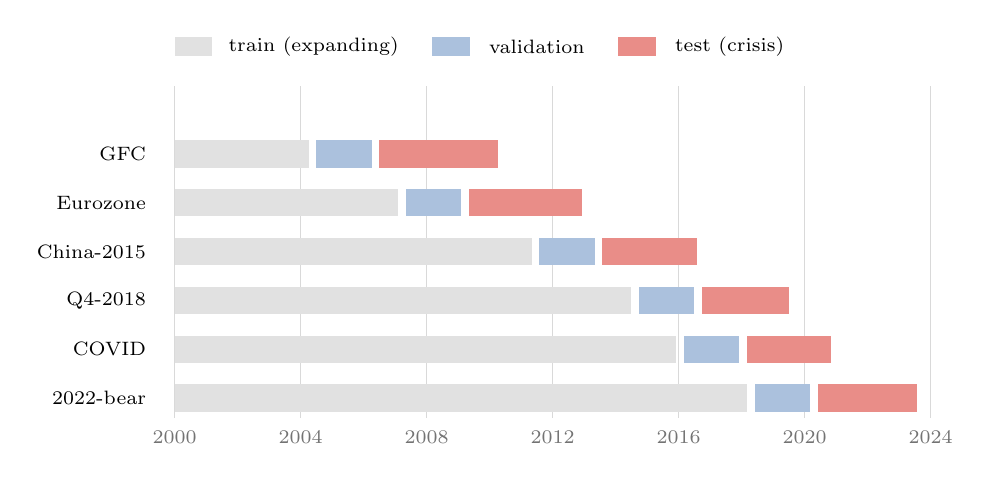
\begin{tikzpicture}[x=0.40cm,y=0.62cm]
  % time axis 2000..2024
  \foreach \yr in {2000,2004,...,2024} {
    \pgfmathsetmacro\xx{(\yr-2000)}
    \draw[black!15] (\xx,-0.4) -- (\xx,6.4);
    \node[font=\scriptsize,black!55] at (\xx,-0.8) {\yr};
  }
  % rows: fold name + train(grey) / val(blue) / test(red) bands by year offset
  % data: fold / train_end / val_start / val_end / test_start / test_end (decimal yr from 2000)
  \foreach \name/\trend/\vst/\vend/\tst/\tend/\row in {
    GFC/4.25/4.5/6.25/6.5/10.25/5,
    Eurozone/7.08/7.33/9.08/9.33/12.92/4,
    China-2015/11.33/11.58/13.33/13.58/16.58/3,
    Q4-2018/14.5/14.75/16.5/16.75/19.5/2,
    COVID/15.92/16.17/17.92/18.17/20.83/1,
    2022-bear/18.17/18.42/20.17/20.42/23.58/0} {
    \node[font=\scriptsize,anchor=east] at (-0.6,\row) {\name};
    \fill[bandgrey] (0,\row-0.28) rectangle (\trend,\row+0.28);
    \fill[regblue!45] (\vst,\row-0.28) rectangle (\vend,\row+0.28);
    \fill[crisisred!55] (\tst,\row-0.28) rectangle (\tend,\row+0.28);
  }
  % legend: each swatch is placed relative to the preceding label's east edge,
  % so it can never ride over that text however wide the text sets.
  \fill[bandgrey] (0,7.0) rectangle (1.2,7.4);
  \node[font=\scriptsize,anchor=west] (lgtrain) at (1.4,7.2) {train (expanding)};
  \node[font=\scriptsize,anchor=west] (lgval) at ([xshift=9mm]lgtrain.east) {validation};
  \fill[regblue!45] ([xshift=-6mm,yshift=-1.24mm]lgval.west)
              rectangle ([xshift=-1.2mm,yshift=1.24mm]lgval.west);
  \node[font=\scriptsize,anchor=west] (lgtest) at ([xshift=9mm]lgval.east) {test (crisis)};
  \fill[crisisred!55] ([xshift=-6mm,yshift=-1.24mm]lgtest.west)
                rectangle ([xshift=-1.2mm,yshift=1.24mm]lgtest.west);
\end{tikzpicture}
\caption{Crisis-anchored walk-forward folds with 63-day embargo. Each row is
one fold; grey is the expanding training history, blue the calm validation
window, red the crisis test window. The small gaps between blocks are the
embargo (purged label-horizon rows). Exact date ranges are listed in
Table~\ref{tab:folddates} (Appendix~\ref{app:folds}).}
\label{fig:cv}
\end{figure}

\subsection{Model: TFT backbone and the AF recipe}
\label{sec:method-model}
The backbone is the TFT of \citet{lim2021tft}: per-time-step variable
selection networks (VSN) weight the inputs; a sequence-to-sequence LSTM
encoder/decoder produces context; static-context GRNs (active only in the
panel) inject the market embedding; an interpretable multi-head attention
block mixes long-range temporal context; and gated residual networks (GRN)
with skip connections carry information around each sub-layer. We replace the
quantile-forecast head with a sigmoid classification head for the binary EWS
target. Figure~\ref{fig:arch} shows the backbone (black) with our two
modifications (green) and the regime branch we tested and rejected (blue,
dashed).

\paragraph{The AF recipe (our contribution).} Two changes to the
\emph{learning problem}, not the backbone topology.

\emph{(1) Auxiliary forward-drawdown head.} A linear head maps each decoder
step's representation $\mathbf{z}_{t+h}\in\mathbb{R}^{s}$ to a scalar
$\hat d_{m,t,h}=\mathbf{w}^{\top}\mathbf{z}_{t+h}+b$ predicting the
\emph{forward running drawdown} at that step. The target is the realised
running drawdown over the decoder horizon,
\begin{equation}
d_{m,t,h}\;=\;D_{m,t+h}\;=\;\frac{X_{m,t+h}}{P_{m,t+h}}-1\;\le 0,
\qquad h=1,\dots,63,
\label{eq:auxtarget}
\end{equation}
i.e.\ the same trailing-252-day-peak drawdown used for labelling
(Eq.~\ref{eq:label}), as a raw (unstandardised, signed) fraction. Unlike the
sparse binary onset label, this target is defined on \emph{every} forward day
(including in-crisis days), supplying a dense regression signal that
regularises the shared representation; it is used only in training. The
auxiliary loss is the mean squared error over the decoder window,
$\mathcal{L}_{\mathrm{aux}}=\frac{1}{63}\sum_{h=1}^{63}(\hat d_{m,t,h}-d_{m,t,h})^2$.

\emph{(2) Focal loss} \citep{lin2017focal} on the onset head, which
down-weights easy negatives so the gradient concentrates on the rare positives.
With probability $p=\sigma(\ell)$ for logit $\ell$, label $y$, and the
true-class probability $p_t=yp+(1{-}y)(1{-}p)$,
\begin{equation}
\mathcal{L}_{\mathrm{focal}}=-\,(1-p_t)^{\gamma}\,
\big[\,w_{+}\,y\log p+(1-y)\log(1-p)\,\big],
\label{eq:focal}
\end{equation}
i.e.\ the standard focal loss with the rare positive class up-weighted by
$w_{+}$; the modulating factor $(1-p_t)^{\gamma}$ is clipped below at
$\epsilon=10^{-6}$ for numerical stability, $\gamma=2$ is the focusing
parameter, and $\gamma=0$ recovers weighted BCE. The full objective is
\begin{equation}
\mathcal{L}=\beta\,\mathcal{L}_{\mathrm{focal}}
+\lambda\,\mathcal{L}_{\mathrm{aux}}
+\gamma_{\mathrm{reg}}\,\mathcal{L}_{\mathrm{regime}},
\label{eq:loss}
\end{equation}
with $\beta=1$, $\lambda=0.5$, and $w_{+}$ set near the inverse prevalence
($3.4$ single-market, $2.5$ panel). For the AF model the regime term is off
($\gamma_{\mathrm{reg}}=0$); the regime variant below sets
$\gamma_{\mathrm{reg}}=0.3$. ``AFv2'' is AF with panel-matched capacity
(hidden/state size $128$), $60$ epochs, learning rate $5\times10^{-4}$, and
per-market normalisation.

\paragraph{The regime branch (tested, inert).} For completeness we also
implement a differentiable neural-HMM \emph{regime module} with $K=3$ latent
states (calm/stress/crisis) on top of the LSTM hidden states
$\mathbf{h}_{1:T}$, plus a \emph{regime-conditioned attention bias}. The module
produces per-step emission log-likelihoods from a gated residual network and a
\emph{time-varying} row-stochastic transition matrix from an MLP,
\begin{equation}
\mathbf{e}_t=\log\mathrm{softmax}\big(\mathrm{GRN}(\mathbf{h}_t)\big),\qquad
A_t=\mathrm{softmax}_{\mathrm{row}}\big(\mathrm{MLP}(\mathbf{h}_t)\big)\in\mathbb{R}^{K\times K},
\end{equation}
where the MLP bias is initialised to a sticky diagonal ($+3$ on, $-3$ off, so
each row starts $\approx[0.9500,0.0250,0.0250]$). Filtered posteriors
$\boldsymbol\pi_t$ are obtained by the differentiable forward algorithm in
log-space,
\begin{equation}
\log\alpha_t=\Big(\operatorname*{logsumexp}_{k'}\big[\log\alpha_{t-1}+\log A_{t-1}\big]\Big)+\mathbf{e}_t,
\quad
\boldsymbol\pi_t=\mathrm{softmax}(\log\alpha_t),
\end{equation}
initialised at $\log\alpha_1=\log\boldsymbol\pi_0+\mathbf{e}_1$. The regime
posteriors over the decoder steps add a learned bias
$b_{\boldsymbol\pi_i,\boldsymbol\pi_j}$ (a $K\times K\times H$ tensor over
query-regime, key-regime, and head, with $H$ attention heads) to the attention
logits, and a label-smoothed NLL term $\mathcal{L}_{\mathrm{regime}}$ supervises
the posteriors against a three-state regime label (calm $=0$; stress $=1$ when
$\mathrm{VIX}\ge 25$ and not in crisis; crisis $=2$ when the trailing-peak
drawdown $\ge 20\%$) and enters Eq.~\ref{eq:loss}. The regime
attention is a no-op without the module, so the ablation cells
(Section~\ref{sec:res-regime}) are nested rather than fully factorial.
Section~\ref{sec:res-regime} reports that none of this improves on the vanilla
backbone.

\begin{figure}[t]
\centering
% The diagram sets ~18.1cm wide against a 16.2cm text block. An over-wide box
% cannot shrink \centering's flush glue, so it pins to the left margin and
% spills into the right one; scaling it to \textwidth makes it fit and centre.
\resizebox{\textwidth}{!}{%
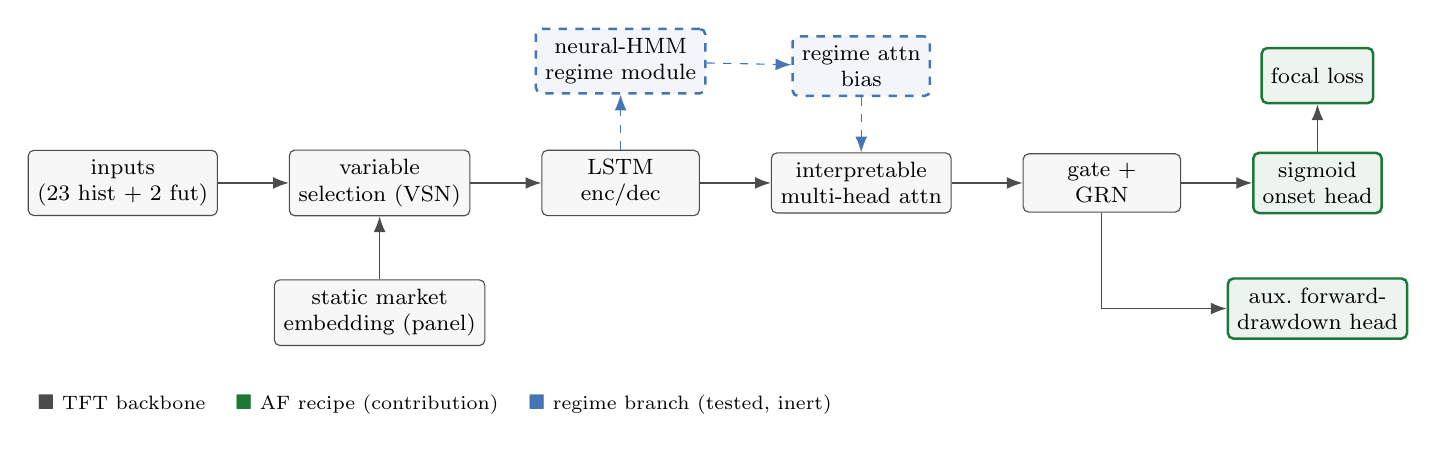
\begin{tikzpicture}[
  font=\footnotesize,
  box/.style={draw=black!70,rounded corners=2pt,minimum height=7mm,minimum width=20mm,align=center,fill=black!3},
  add/.style={draw=addgreen,line width=0.9pt,rounded corners=2pt,minimum height=7mm,align=center,fill=addgreen!8},
  reg/.style={draw=regblue,dashed,line width=0.9pt,rounded corners=2pt,minimum height=7mm,align=center,fill=regblue!7},
  ar/.style={-{Latex[length=2mm]},black!70},
  node distance=6mm and 9mm,
]
\node[box] (inp) {inputs\\(23 hist + 2 fut)};
\node[box,right=of inp] (vsn) {variable\\selection (VSN)};
\node[box,right=of vsn] (lstm) {LSTM\\enc/dec};
\node[box,right=of lstm] (attn) {interpretable\\multi-head attn};
\node[box,right=of attn] (grn) {gate +\\GRN};
\node[add,right=of grn] (head) {sigmoid\\onset head};
\draw[ar] (inp)--(vsn); \draw[ar] (vsn)--(lstm); \draw[ar] (lstm)--(attn);
\draw[ar] (attn)--(grn); \draw[ar] (grn)--(head);
% static (panel only)
\node[box,below=8mm of vsn] (stat) {static market\\embedding (panel)};
\draw[ar] (stat)--(vsn);
% AF additions
\node[add,below=8mm of head] (aux) {aux.\ forward-\\drawdown head};
\draw[ar] (grn)|-(aux);
\node[add,above=6mm of head,align=center] (focal) {focal loss};
\draw[ar] (head)--(focal);
% regime branch (rejected)
\node[reg,above=7mm of lstm] (hmm) {neural-HMM\\regime module};
\node[reg,above=7mm of attn] (bias) {regime attn\\bias};
\draw[ar,regblue,dashed] (lstm)--(hmm); \draw[ar,regblue,dashed] (hmm)--(bias);
\draw[ar,regblue,dashed] (bias)--(attn);
% legend (placed below the lowest boxes to avoid overlap)
\node[align=left,anchor=north west,font=\scriptsize] at ($(inp.west |- stat.south)+(0,-0.5)$)
 {\textcolor{black!70}{$\blacksquare$} TFT backbone \quad
  \textcolor{addgreen}{$\blacksquare$} AF recipe (contribution) \quad
  \textcolor{regblue}{$\blacksquare$} regime branch (tested, inert)};
\end{tikzpicture}%
}
\caption{Model overview. Black: the TFT backbone \citep{lim2021tft}. Green:
the AF recipe, a multi-task auxiliary forward-drawdown head and focal loss
(Eq.~\ref{eq:loss}), which is the contribution. Blue/dashed: the neural-HMM
regime module and regime-conditioned attention bias, implemented and ablated
but found inert.}
\label{fig:arch}
\end{figure}

\subsection{Training and evaluation}

\paragraph{The metrics in plain terms.} Because the evidence in
Section~\ref{sec:results} rests on a few recurring measures, we state them once
in words. \emph{Prevalence} $\pi$ is the fraction of test days that are
positive (here $\pi\approx0.34$); a model that guesses at random scores about
$\pi$, so $\pi$ is the ``no-skill'' floor. \emph{PR-AUC} (area under the
precision--recall curve, $0$--$1$, higher better) summarises how well the model
ranks true crisis days above calm ones; unlike accuracy it stays meaningful
when positives are rare, and it must be read against $\pi$, so a PR-AUC of
$0.48$ against a $0.34$ floor is real skill, not near-perfect. \emph{Skill}
$=(\prauc-\pi)/(1-\pi)$ simply rescales this so $0=$ no better than the floor
and $1=$ perfect. \emph{ROC-AUC} is a related ranking score (chance $=0.50$)
that, unlike PR-AUC, is insensitive to how rare crises are; we report it for
completeness but treat PR-AUC as primary
\citep{saito2015prc}. \emph{Calibration} asks whether a stated, say, $30\%$
chance of crisis really does occur about $30\%$ of the time; the \emph{Brier
score} (mean squared error of the probabilities, lower better) measures it, and
\emph{Platt scaling} is a light post-processing step that rescales raw
probabilities to be better calibrated (``Platt'' columns are after this step).
Scores are \emph{macro-averaged}: computed per crisis fold, then averaged, so
each crisis counts equally regardless of its length.

\paragraph{Protocol.}
Optimisation uses AdamW with gradient clipping; the best checkpoint is selected
on validation $\prauc$ (not validation loss, which rises monotonically here
and would select an under-trained epoch). Determinism is hardened
(seeded data loaders, exported \texttt{CUBLAS\_WORKSPACE\_CONFIG}, A100-pinned
runs). The primary metric is $\prauc$ (also reported as skill over the
prevalence baseline); we also report $\rocauc$, the Brier score, and post-hoc
Platt calibration. Each configuration is run over up to 30 seeds and six folds.
\emph{Seeds estimate run-to-run variability of the stochastic neural models;
they are not independent observations of market crises.} Primary inference is
therefore conducted at the \emph{crisis-episode} level: we average over seeds
within each fold and compare models across the six folds (Wilcoxon signed-rank
and a block bootstrap that resamples episodes). Seed$\times$fold tests are
reported only as sensitivity diagnostics, never as headline claims, because,
with only $\sim$6 crisis episodes, statistical power is bounded by episode
count, not seed count (Section~\ref{sec:res-regime}).

% =====================================================================
\section{Experiments and Results}
\label{sec:results}

All numbers below use the leak-free protocol of Section~\ref{sec:method-cv}.
We report the single-market study first (backbone, regime ablation, loss/AF
study, threshold sensitivity, calibration), then the panel study, then the
transfer of the unified recipe.

\subsection{Backbone: TFT beats LSTM and XGBoost on clean splits}
\label{sec:res-backbone}
On the embargoed walk-forward splits the TFT backbone is the clear winner
among single-market models (Table~\ref{tab:backbone}), under the \emph{same}
six-fold, $\approx$30-seed protocol as the headline results (so the vanilla TFT
figure matches Table~\ref{tab:af}). An earlier, leakage-contaminated pipeline
had reported LSTM ahead of TFT; once the target leak, the all-time-peak
labelling bug, and the validation-loss checkpoint bug are fixed, the ranking is
TFT $>$ LSTM $>$ XGBoost. This justifies TFT as the backbone.

\begin{table}[h]
\centering\small
\caption{Single-market backbone comparison, macro $\prauc$ over the six
embargoed crisis-anchored walk-forward folds ($\approx$30 seeds for the
neural models; XGBoost deterministic), prevalence $\pi=0.3358$. Same
protocol as Table~\ref{tab:af}.}
\label{tab:backbone}
\begin{tabular}{lc}
\toprule
Model & Macro $\prauc$ \\
\midrule
\textbf{Vanilla TFT} & \textbf{0.4592} \\
LSTM & 0.3465 \\
XGBoost & 0.3370 \\
\bottomrule
\end{tabular}
\end{table}

\paragraph{The trees are not crippled.} To ensure the deep advantage is not an
artefact of weak baselines, we ran a hyperparameter grid (three configurations
each) for XGBoost, Random Forest, and histogram gradient boosting (a
LightGBM-style sklearn model). All three trees receive the identical flattened
input window as the deep models. Selecting the grid on validation PR-AUC is not
possible here: as noted in Section~\ref{sec:res-af}, four of the six validation
splits contain no positive labels, so no validation ranking metric exists for
them. We therefore report, for each model and fold, the \emph{best of the three
configurations scored on the test fold itself} (Table~\ref{tab:trees}). This is
deliberately generous: it is an optimistic upper bound that gives the trees an
advantage no honest protocol would grant them, since the configuration is
chosen with knowledge of the very set it is scored on. Even so, the best tree
(Random Forest, $0.3566$) remains far below the deep models
($0.4592$--$0.4869$), and the $\approx$$0.13$ gap survives tuning. The trees
win only on mild corrections (e.g.\ Q4-2018) and lose heavily on the severe,
volatile crises where the deep models excel (Appendix~\ref{app:perfold}). On
GFC and Eurozone every tree configuration collapses to the fold prevalence
($0.2725$ and $0.2843$), that is, to a constant prediction with no skill at
all.

\begin{table}[h]
\centering\small
\caption{Tuned tree baselines vs.\ deep models, macro $\prauc$ over the six
folds. Each tree row is the \emph{best of a three-configuration grid scored on
the test fold itself}, an optimistic upper bound adopted because four of the
six validation splits contain no positive labels and therefore admit no
validation ranking metric (Section~\ref{sec:res-af}); all trees use the same
flattened input window as the deep models. The two deep rows are the same
conf-M0/AF runs as the headline Table~\ref{tab:af} and are \emph{not}
test-selected.}
\label{tab:trees}
\begin{tabular}{lcc}
\toprule
Model & Macro $\prauc$ & Macro Brier $\downarrow$ \\
\midrule
\textbf{AF (deep)}        & \textbf{0.4869} & \textbf{0.2703} \\
Vanilla TFT (deep)        & 0.4592 & 0.3173 \\
Random Forest (test-selected)     & 0.3566 & 0.3037 \\
XGBoost (test-selected)           & 0.3399 & 0.3866 \\
HistGradientBoosting (test-selected) & 0.3334 & 0.3756 \\
\bottomrule
\end{tabular}
\end{table}

\subsection{Regime awareness is inert}
\label{sec:res-regime}
We ablate the regime machinery factorially: M0 (vanilla TFT), M1 (module
present but unused), M2 ($+$ regime aux loss), M3 ($+$ regime attention), M4
(full RA-TFT). Table~\ref{tab:regime} (3-fold exploratory run) shows that no
single component helps, M1$\approx$M0, M2 and M3 fall \emph{below} M0, and
only the full M4 combination edges above vanilla, by a small interaction
effect. A 30-seed, six-fold confirmatory run settles the question:

\begin{center}
\emph{Full RA-TFT vs.\ vanilla TFT: macro $\prauc$ $0.4630$ vs.\ $0.4592$;
paired Wilcoxon $p=0.4375$ (n.s.).}
\end{center}

\begin{table}[h]
\centering\small
\caption{Regime ablation (single-market, exploratory 3-fold, macro $\prauc$
raw / Platt). No component helps in isolation; only the full stack (M4)
marginally exceeds vanilla, and the effect is not significant under the
powered run.}
\label{tab:regime}
\begin{tabular}{llc}
\toprule
Cell & Description & raw $\prauc$ \\
\midrule
M0 & vanilla TFT & 0.5274 \\
M1 & regime module present, unused & 0.5221 \\
M2 & $+$ regime auxiliary loss & 0.5106 \\
M3 & $+$ regime attention bias & 0.4754 \\
M4 & full RA-TFT & 0.5546 \\
\bottomrule
\end{tabular}
\end{table}

\paragraph{Seeds cannot rescue it.} Increasing from 10 to 30 seeds barely
moved the $p$-value ($0.0822\to0.0783$ on the three-fold confirmatory run). The
reason is structural: the variance that matters is \emph{between crisis
episodes} (e.g.\ COVID is easy, the GFC fold is hard), and with only six
episodes the test has little power regardless of seeds. The point is worth
stating plainly: \emph{more seeds cannot establish significance for regime
awareness; only more independent crises could}, and the data barely stretch to
six. That is the central caveat of the whole study. The regime module is a
well-motivated idea that does not survive a powered, leak-free test.

\subsection{What works: the AF recipe}
\label{sec:res-af}
Searching over loss/objective choices on the embargoed splits, focal loss with
$w_{+}=3.4$ is the best loss, and adding the auxiliary forward-drawdown head
on top (the AF recipe) is the best configuration overall on every aggregate
metric. Table~\ref{tab:af} reports the six-fold confirmatory comparison.
How we test it matters here: the independent unit
of evidence is the crisis episode (six folds), not the random seed, so we
report effect sizes and episode-level uncertainty rather than a seed-level
$p$-value (see \emph{Why not the seed-level $p$-value} at the end of this
section).

\begin{table}[h]
\centering\small
\caption{Single-market headline. \emph{Protocol:} S\&P~500, dd10 threshold,
six crisis-anchored walk-forward folds, $\approx$30 seeds per fold; each cell
is the mean over folds of the per-seed mean (macro-averaging), prevalence
baseline $\pi=0.3358$. Brier is lower-is-better; skill is
$(\prauc-\pi)/(1-\pi)$ computed per fold and then macro-averaged. AF $=$ vanilla
TFT $+$ auxiliary forward-drawdown head $+$ focal loss. AF lowers Brier in all
six folds; the $\prauc$ gain is positive but episode-limited
(Section~\ref{sec:res-af}). Post-hoc Platt figures are reported separately
below, because Platt could be fitted on only two of the six folds.}
\label{tab:af}
\begin{tabular}{lccc}
\toprule
Model & raw $\prauc$ & Brier $\downarrow$ & skill \\
\midrule
M0 (vanilla TFT)        & 0.4592 & 0.3173 & 0.1562 \\
M4 (full RA-TFT)        & 0.4630 & 0.3041 & 0.1655 \\
\textbf{AF (aux+focal)} & \textbf{0.4869} & \textbf{0.2703} & \textbf{0.1947} \\
\bottomrule
\end{tabular}
\end{table}

\paragraph{A note on post-hoc calibration.} Platt scaling is fitted on the
validation split, and in four of the six folds (GFC, Eurozone, China-2015 and
Q4-2018) that split contains \emph{no positive labels at all}: the validation
window falls in a calm stretch, so the positive rate is exactly zero and the
scaling cannot be fitted. Platt figures therefore exist only for COVID and
2022-bear, and are reported here for those two folds alone rather than beside
the six-fold columns of Table~\ref{tab:af}, where they would invite a false
comparison. Over those two folds the Platt $\prauc$ is $0.5451$ (M0), $0.6232$
(M4) and $0.6560$ (AF), and the Platt Brier is $0.2845$, $0.2699$ and $0.2393$
respectively. The apparent lift over the raw six-fold $\prauc$ is an artefact
of the fold subset, not of the scaling: Platt is monotonic, so it cannot change
$\prauc$ at all, and indeed on 2022-bear the Platt and raw values agree to six
decimal places. The absence of validation positives in four folds is a real
limitation of the crisis-anchored design and is revisited in
Section~\ref{sec:limits}.

\paragraph{Calibration: a consistent, unambiguous gain.} The clearest result
needs no significance test: AF lowers the Brier score in \emph{every one of
the six crisis folds} (Table~\ref{tab:af}, macro $0.2703$ vs.\ $0.3173$), with
per-fold reductions ranging from $0.0158$ (Eurozone) to $0.0906$
(China-2015). Dense drawdown supervision yields probabilities a downstream risk
rule can trust, and this benefit is uniform across crises rather than
concentrated.

\paragraph{Discrimination: a positive but episode-limited effect.} On
$\prauc$, AF improves the macro average by $+0.0315$ and wins four of six
folds, but the effect is \emph{concentrated} in severe, volatile regime-shift
crises and is small or slightly negative on mild corrections
(Figure~\ref{fig:perfold}): COVID $+0.1613$ and China-2015 $+0.0405$ dominate,
while Q4-2018 ($-0.0195$) and 2022 ($-0.0118$) are flat. Throughout, we quote this
gain as the \emph{seed-paired} mean difference: we difference AF and vanilla
\emph{within} each seed and then average, which cancels the run-to-run noise
common to both models and is the quantity the tests below are computed on. It
is therefore not identical to subtracting the two macro rows of
Table~\ref{tab:af} ($0.4869-0.4592=+0.0277$), because seed coverage differs
slightly across cells after pre-emption; the two agree to $0.0038$. Treating
the six crisis episodes as the independent unit, this improvement is
\emph{not} statistically significant (Wilcoxon signed-rank over folds
$p=0.5625$; sign test $p=0.6875$), and a block bootstrap resampling crisis
episodes gives a 95\% confidence interval for the macro gain of
$[-0.0069,\,+0.0858]$ that narrowly includes zero (probability of a positive
effect $0.9140$). We therefore claim a \emph{consistent improvement concentrated
where it matters most (real crises)}, not a proven discrimination gain. The
paragraph below explains why a seed-level test would overstate this.

\paragraph{Why not the seed-level \emph{p}-value.}
A paired Wilcoxon over all $\approx$170 seed$\times$fold pairs returns
$p=0.0231$, which looks decisive but is \emph{pseudo-replicated}: thirty random
initialisations of the same six crises are not thirty independent crisis
observations, and the small $p$ is driven almost entirely by the single large
COVID effect being repeated across correlated seeds. The right unit is the
crisis episode, of which we have six; as the regime analysis already noted
(Section~\ref{sec:res-regime}), no amount of seeds can manufacture power that
only more independent crises could provide. We quote the seed-level number
once, here, to flag the discrepancy, and base every discrimination claim on the
episode-level statistics above.

\begin{figure}[t]
\centering
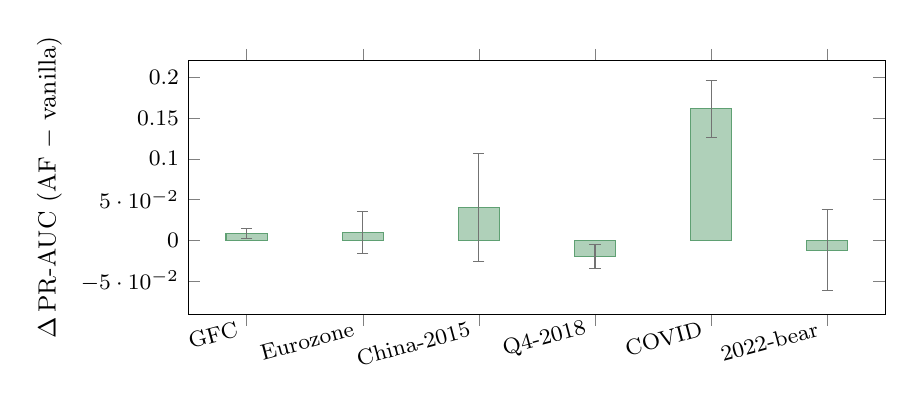
\begin{tikzpicture}
\begin{axis}[
  width=0.86\textwidth, height=4.8cm,
  ybar, bar width=15pt,
  ymin=-0.09, ymax=0.22,
  symbolic x coords={GFC,Eurozone,China-2015,Q4-2018,COVID,2022-bear},
  xtick=data, x tick label style={font=\footnotesize,rotate=15,anchor=east},
  ylabel={$\Delta\,\prauc$ (AF $-$ vanilla)}, label style={font=\small},
  ytick={-0.05,0,0.05,0.10,0.15,0.20}, tick label style={font=\footnotesize},
  enlarge x limits=0.10,
]
\addplot+[draw=addgreen!70,fill=addgreen!35,
          error bars/.cd, y dir=both, y explicit,
          error bar style={black!55}] coordinates {
  (GFC,0.0085)        +- (0,0.0060)
  (Eurozone,0.0102)   +- (0,0.0256)
  (China-2015,0.0405) +- (0,0.0663)
  (Q4-2018,-0.0195)   +- (0,0.0147)
  (COVID,0.1613)      +- (0,0.0350)
  (2022-bear,-0.0118) +- (0,0.0495)};
\end{axis}
\end{tikzpicture}
\caption{Per-fold improvement of AF over vanilla TFT in $\prauc$ (AF $-$
vanilla, differenced within each seed and then averaged over seeds, so that
run-to-run noise common to both models cancels). The gain concentrates in the
severe COVID ($+0.1613$) and China-2015 ($+0.0405$) regime-shift crises and is
small or slightly negative on mild corrections (Eurozone $+0.0102$, GFC
$+0.0085$, 2022 $-0.0118$, Q4-2018 $-0.0195$). Error bars are $\pm1$ standard
error across seeds (run-to-run); single-crisis estimates are highly variable
(seed SD up to $0.3511$), and the dominant uncertainty is \emph{between}
crises; the episode-level bootstrap CI is $[-0.0069,+0.0858]$
(Section~\ref{sec:res-af}).}
\label{fig:perfold}
\end{figure}

\paragraph{What else we tried and dropped.} Monte-Carlo dropout gave no
calibration benefit (slight $\prauc$ cost); a regime-conditioned VSN was not
significant; $K=3$ latent regime states was best ($K=5$ significantly worse);
and $\gamma\in\{2,3\}$ was the best focal focusing range. None of these
changed the headline.

\subsection{Isolating the contribution: which head does the work?}
\label{sec:res-heads}
The AF recipe of Section~\ref{sec:res-af} changes two things at once relative
to the vanilla baseline: it adds the auxiliary drawdown head, and it swaps
weighted BCE for focal loss with $w_{+}=3.4$. A comparison against M0
therefore cannot say which ingredient is responsible, and it leaves open a
more basic question: if a drawdown regressor is useful, is the classification
head needed at all, or would simply \emph{replacing} it suffice? We resolve
both with a three-way ablation in which the only thing that varies is which
head or heads exist. All three cells share the same backbone with the regime
branch explicitly disabled, and every cell that contains a classification term
uses the identical focal objective, so the loss is held fixed wherever it is
present:

\begin{itemize}\itemsep2pt
\item \textbf{CLF-only} --- classification head alone, focal loss with
      $w_{+}=3.4$. This is the control the AF-versus-M0 comparison lacks.
\item \textbf{Both heads} --- classification head plus the auxiliary
      forward-drawdown head; the AF recipe, with the regime branch off.
\item \textbf{REG-only} --- the drawdown head alone. The classification term is
      removed from the objective entirely ($\beta=0$), so only the regression
      loss trains, and the crisis score is read from the regression output.
\end{itemize}

Scoring REG-only requires care. The regression head emits a drawdown, not a
probability, and the sign of its relationship to the crisis label is not fixed:
among calm anchors a deeper drawdown indicates elevated risk, whereas over the
full test population --- which retains windows already inside a crisis --- the
relationship inverts, because a deep drawdown there marks a crash that has
already happened rather than one about to begin. Assuming either direction
would risk manufacturing the result. We therefore fit a one-dimensional
logistic map from predicted drawdown to crisis probability on the
\emph{training} split alone, so the direction is learned rather than imposed,
and we additionally record the raw predictions so that every REG-only model can
be re-scored under the opposite sign. Checkpoint selection for this cell uses
its own regression objective, since a classification metric would be
meaningless for a head that receives no gradient.

\begin{table}[h]
\centering\small
\caption{Head ablation. \emph{Protocol:} S\&P~500, dd10, six crisis-anchored
walk-forward folds, 30 seeds per fold, regime branch disabled throughout,
prevalence baseline $\pi=0.3358$. CLF-only and Both-heads share the identical
focal objective, so the single difference between them is the auxiliary head.
M0 is carried over from Table~\ref{tab:af} as the untuned reference. Brier is
lower-is-better.}
\label{tab:heads}
\begin{tabular}{lccc}
\toprule
Configuration & raw $\prauc$ & Brier $\downarrow$ & skill \\
\midrule
M0 (vanilla TFT, weighted BCE)   & 0.4592 & 0.3173 & 0.1562 \\
CLF-only (focal, no aux head)    & 0.4521 & 0.2853 & 0.1448 \\
\textbf{Both heads (AF)}         & \textbf{0.4852} & 0.2791 & \textbf{0.1913} \\
REG-only (drawdown head alone)   & 0.3649 & \textbf{0.2494} & 0.0365 \\
\bottomrule
\end{tabular}
\end{table}

\paragraph{The auxiliary head, not the loss, carries the recipe.} Holding the
objective fixed, adding the drawdown head improves macro $\prauc$ by
$+0.0342$ and does so in \emph{all six} crisis folds
(Figure~\ref{fig:heads}). Under the episode-level treatment this report argues
for throughout, that is a Wilcoxon signed-rank $p=0.0312$ --- with six
episodes, six wins out of six is the smallest two-sided $p$-value the test can
return --- and a block bootstrap over crisis episodes gives a 95\% confidence
interval for the macro gain of $[+0.0133,\,+0.0595]$, which excludes zero
(probability of a positive effect $1.0000$). This is a materially stronger
statement than the headline of Section~\ref{sec:res-af}, whose interval
$[-0.0069,+0.0858]$ narrowly included zero, and it is obtained on the
conservative unit of analysis rather than the pseudo-replicated seed-level one
(the seed$\times$fold test, quoted once for comparison, gives $p=0.0030$).

The reason the earlier comparison was weaker is now visible: the focal loss
contributes nothing. CLF-only differs from M0 only in the objective, and it is
$-0.0045$ macro $\prauc$ \emph{below} it, winning three folds of six
(Wilcoxon $p=1.0000$; seed$\times$fold $p=0.6042$). The loss change that the
exploratory sweep of Section~\ref{sec:res-threshold} favoured does not survive at six
folds and thirty seeds. Attributing the AF gain to ``aux $+$ focal'' therefore
credits an inert ingredient; the auxiliary head accounts for the whole effect.
Consistent with Section~\ref{sec:res-regime}, disabling the regime branch inside
the AF cell changes macro $\prauc$ by $0.0017$ ($0.4852$ against $0.4869$),
confirming once more that the regime machinery is inert.

\paragraph{The classification head cannot simply be replaced.} REG-only is far
weaker at discrimination: macro $\prauc$ $0.3649$ against a prevalence
baseline of $0.3358$, a skill of $0.0365$ where the two-head model reaches
$0.1913$. Re-scoring the identical models under the opposite sign gives
$0.4224$, still below every configuration that retains a classification head,
and the favoured direction is not even consistent across folds --- the fitted
direction wins on GFC and COVID while the inverted one wins on Eurozone,
Q4-2018 and 2022-bear. Even an oracle permitted to choose the better sign per
fold in hindsight reaches only $\approx0.47$, short of the two-head model's
$0.4852$. The answer to whether a head swap would suffice is therefore no: the
drawdown signal is a useful auxiliary target but an unreliable classifier in
its own right.

\paragraph{Why the second head helps.} The per-fold pattern explains the
mechanism rather than merely recording it. REG-only outperforms every
classification-based configuration on exactly the two folds where those
configurations fall \emph{below their own prevalence baseline}: GFC
($0.3642$ against $0.2172$--$0.2335$, baseline $0.2725$) and Q4-2018
($0.5306$ against $0.4019$--$0.4315$, baseline $0.5710$). GFC is the extreme
case, because its training window contains no positive labels whatsoever
(Section~\ref{sec:limits}), so the binary target supplies nothing for a
classifier to learn from. The drawdown target, by contrast, is defined on
every trading day. Where crisis labels are abundant the ordering reverses
sharply and the classifier dominates --- COVID $0.7935$ against $0.5220$,
China-2015 $0.4561$ against $0.2828$. Dense supervision is thus not a
general-purpose substitute for the discriminative signal; it is a complement
that supplies gradient precisely in the label-starved regime where sparse
crisis targets fail, which is why the two heads together beat either alone.
This is the mechanism behind the calibration result of
Section~\ref{sec:res-af}, and it is also why REG-only attains the best Brier
score of any cell ($0.2494$) while being the weakest at ranking: a regression
head produces conservative, well-spread probabilities, but conservative
probabilities and good discrimination are not the same property.

\begin{figure}[t]
\centering
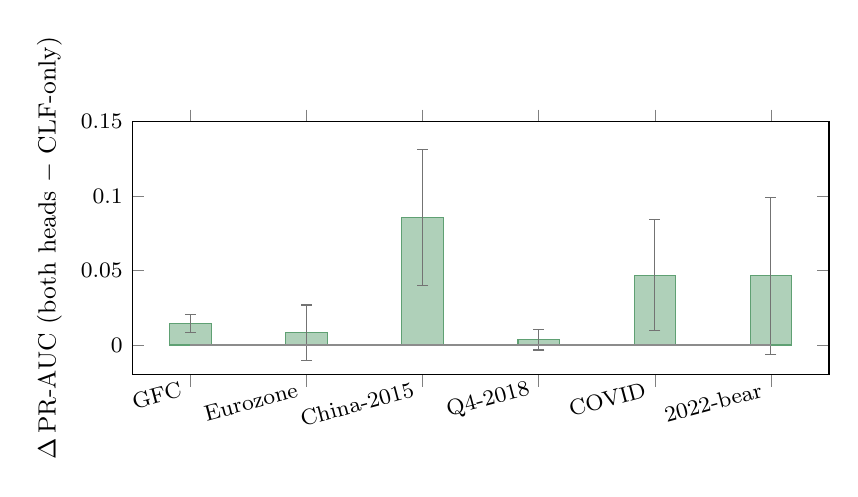
\begin{tikzpicture}
\begin{axis}[
  width=0.86\textwidth, height=4.8cm,
  ybar, bar width=15pt,
  ymin=-0.02, ymax=0.15,
  symbolic x coords={GFC,Eurozone,China-2015,Q4-2018,COVID,2022-bear},
  xtick=data, x tick label style={font=\footnotesize,rotate=15,anchor=east},
  ylabel={$\Delta\,\prauc$ (both heads $-$ CLF-only)}, label style={font=\small},
  ytick={0,0.05,0.10,0.15}, tick label style={font=\footnotesize},
  scaled y ticks=false,
  y tick label style={font=\footnotesize, /pgf/number format/fixed,
                      /pgf/number format/precision=2},
  enlarge x limits=0.10,
]
\addplot+[draw=addgreen!70,fill=addgreen!35,
          error bars/.cd, y dir=both, y explicit,
          error bar style={black!55}] coordinates {
  (GFC,0.0144)        +- (0,0.0058)
  (Eurozone,0.0083)   +- (0,0.0186)
  (China-2015,0.0856) +- (0,0.0457)
  (Q4-2018,0.0036)    +- (0,0.0069)
  (COVID,0.0468)      +- (0,0.0372)
  (2022-bear,0.0464)  +- (0,0.0527)};
\addplot[black!45,sharp plot,update limits=false]
  coordinates {(GFC,0) (2022-bear,0)};
\end{axis}
\end{tikzpicture}
\caption{Effect of adding the auxiliary drawdown head with the loss held
fixed: per-fold $\prauc$ difference between the two-head model and the
classification-only control, differenced within each seed and then averaged
over seeds. Every one of the six crisis folds improves (macro $+0.0342$;
episode-level Wilcoxon $p=0.0312$; bootstrap CI $[+0.0133,+0.0595]$). Unlike
the AF-versus-vanilla comparison of Figure~\ref{fig:perfold}, where the gain
was concentrated in COVID and China-2015 and two folds were negative, the
benefit here is present everywhere, which is what makes the episode-level test
conclusive. Error bars are $\pm1$ standard error across seeds; the dominant
uncertainty remains \emph{between} crises rather than between runs.}
\label{fig:heads}
\end{figure}

\subsection{Calibration and decision usefulness}
\label{sec:res-calib}
Because EWS probabilities feed decisions, we examine calibration directly. A
second calibration metric corroborates the Brier result of
Section~\ref{sec:res-af}: the per-fold-averaged \emph{expected calibration
error} (ECE, ten equal-width bins) is lower for AF than for vanilla TFT
($0.2870$ vs.\ $0.3192$). Figure~\ref{fig:reliability} shows the corresponding
reliability curves: the raw probabilities of \emph{both} models are
over-confident (points below the diagonal at high predicted probability), but
AF lies closer to the diagonal across the operating range. Calibration is thus
the AF recipe's most consistent benefit: it holds in all six folds (Brier) and
on a second, independent metric (ECE).

\begin{figure}[h]
\centering
\begin{tikzpicture}
\begin{axis}[
  width=0.66\textwidth, height=5.2cm,
  xlabel={predicted probability}, ylabel={observed frequency},
  xmin=0, xmax=1, ymin=0, ymax=1,
  tick label style={font=\footnotesize}, label style={font=\small},
  legend pos=north west, legend style={font=\footnotesize, draw=none},
  enlargelimits=false,
]
\addplot[black!40,dashed,thick] coordinates {(0,0) (1,1)};
\addlegendentry{perfect}
\addplot[regblue,thick,mark=*,mark size=1.2pt] table[x=pred,y=obs] {figures/reliability_m0.dat};
\addlegendentry{vanilla TFT (ECE 0.3192)}
\addplot[addgreen,thick,mark=square*,mark size=1.2pt] table[x=pred,y=obs] {figures/reliability_af.dat};
\addlegendentry{AF (ECE 0.2870)}
\end{axis}
\end{tikzpicture}
\caption{Reliability diagram (per-fold-averaged, raw probabilities). Both
models are over-confident relative to the diagonal, motivating the Platt
scaling used in all headline results, but AF (green) is closer to perfect
calibration than vanilla TFT (blue), consistent with its lower ECE and its
lower Brier score in all six folds.}
\label{fig:reliability}
\end{figure}

\paragraph{Cost-sensitive usefulness.} We also computed the cost-sensitive
\emph{usefulness} measure of \citet{sarlin2013biggest}, in which a policymaker
weights missed crises against false alarms through a preference parameter
$\mu$ (higher $\mu$ = more averse to missing a crisis). Writing $T_1$ for the
share of crises missed, $T_2$ for the share of tranquil periods falsely
signalled, and $P_1=\pi$, $P_2=1-\pi$ for the unconditional class
probabilities, the policymaker's loss is
$L(\mu)=\mu T_1 P_1+(1-\mu)T_2 P_2$. The benchmark is the loss of the better
trivial policy, $\min(\mu P_1,\,(1-\mu)P_2)$, achieved by always- or
never-alarming, and relative usefulness is
$U_r=\bigl[\min(\mu P_1,(1-\mu)P_2)-L(\mu)\bigr]/\min(\mu P_1,(1-\mu)P_2)$,
running from $0$ (no better than the trivial policy) to $1$ (perfect). With
the decision threshold chosen at the in-sample optimum, which is an upper bound
on achievable usefulness, AF is more useful than the vanilla TFT at every
preference setting we examined (Table~\ref{tab:useful}), consistent with its
better calibration. Note that under an optimal threshold $U_r$ is bounded below
by zero, because the threshold grid contains the two trivial policies. The
measure itself is not uncontested: \citet{alessidetken2014comment} argue that
normalising by the unconditional crisis probability leaves $U_r$ sensitive to
small perturbations of $\mu$ and awkward to use for policy. That criticism is
why Table~\ref{tab:useful} reports three preference settings rather than one.
The \emph{level} of $U_r$ should not be read too literally, but the ordering is
stable across all three settings, and it is the ordering, not the level, that
the comparison rests on.

\begin{table}[h]
\centering\small
\caption{Sarlin relative usefulness $U_r$ (per-fold-averaged over the six
folds, ten seeds per fold, in-sample optimal threshold, an upper bound).
Higher is better; $\mu$ is the policymaker's aversion to missed crises.}
\label{tab:useful}
\begin{tabular}{lccc}
\toprule
Model & $\mu=0.5$ & $\mu=0.7$ & $\mu=0.9$ \\
\midrule
M0 (vanilla TFT)  & 0.1365 & 0.2674 & 0.2562 \\
\textbf{AF}       & \textbf{0.2008} & \textbf{0.3310} & \textbf{0.3224} \\
\bottomrule
\end{tabular}
\end{table}

More importantly, the \emph{out-of-sample} version, choosing the
threshold on the calm validation window and applying it to the crisis test
window, is \emph{not robustly estimable here}: the pre-crisis validation
windows contain too few onsets to fix a transferable threshold, and where one
exists it transfers poorly across the calm-to-crisis prevalence shift. That is a
finding in its own right about single-market EWS: a fixed alarm threshold set in
quiet times does not carry into a crisis, which is exactly why
\emph{calibrated probabilities} (where AF helps) beat a single hard threshold.

\subsection{Threshold sensitivity}
\label{sec:res-threshold}
The single-market advantage is specific to dd10. Repeating the comparison at
$\tau\in\{12,15,20\}\%$ shows the field collapsing toward a tie as the
threshold rises and episodes become too rare to learn from or evaluate on
(Table~\ref{tab:thr-sens}). This is expected (at dd20 a fold contains
$\sim$1 onset) and it motivates the dd10 operating point. We report it openly
as a limitation rather than tuning the threshold to the result.

\emph{This is a separate, earlier sweep} (a three-fold run of the
regime-aware model on a different harness), used only to study how the
threshold choice affects the deep-vs-tree gap; its ``best deep'' column is
\emph{not} the six-fold AF headline of Table~\ref{tab:af} (whose macro
$\prauc$ is $0.4869$) and the two should not be compared directly. The point of
the table is the \emph{trend} across thresholds, not the level.

\begin{table}[h]
\centering\small
\caption{Threshold-sensitivity sweep (macro $\prauc$, three-fold, regime-aware
deep model; a diagnostic run distinct from the six-fold AF headline of
Table~\ref{tab:af}). ``Best deep'' is the strongest deep configuration in this
sweep at each threshold. The deep-model advantage is strongest at dd10 and
erodes as the threshold rises and events become scarce. (XGBoost not available
at dd12/dd20 in this sweep.)}
\label{tab:thr-sens}
\begin{tabular}{lccc}
\toprule
Threshold & best deep (this sweep) & LSTM & XGBoost \\
\midrule
dd10 & \textbf{0.56} & 0.43 & 0.33 \\
dd12 & 0.35 & \textbf{0.39} & -- \\
dd15 & \textbf{0.36} & 0.33 & 0.35 \\
dd20 & 0.34 & \textbf{0.36} & -- \\
\bottomrule
\end{tabular}
\end{table}

\subsection{Panel: the tuned recipe is competitive with XGBoost}
\label{sec:res-panel}

\paragraph{Panel protocol.} The panel pools the nine indices of
Section~\ref{sec:data} into a single multi-entity dataset, with market identity
as a static categorical consumed by TFT's static encoder (a learned market
embedding). Unlike the single-market study, the panel uses a \emph{single
chronological split shared across all markets}, train to 2015-12-31,
validation to 2018-12-31, test 2019--2026, rather than crisis-anchored
walk-forward folds; a 63-day embargo is applied per market at each boundary,
the feature scaler is fit on the training span only, and windows are built
within each split. Metrics are pooled over all (market, day) test
observations. We first report this pooled chronological split because it
directly tests whether more entities lift deep models above trees at all; we
then subject the same comparison to a five-fold panel walk-forward robustness
check (Table~\ref{tab:panelwf}).

\paragraph{A caveat on ``$\approx$110 episodes''.} The panel contains more
crisis \emph{onsets} than the single market, but they are \emph{not}
independent: the nine indices are highly correlated and most crash together
(e.g.\ COVID is a crisis in all nine within the same weeks), so the effective
number of independent episodes in the 2019--2026 test span is far smaller than
the raw onset count. The panel therefore buys representational variety and
training signal more than it buys independent statistical power, and we treat
its significance tests with the same caution as the single-market ones.

The nine-market panel is harder in absolute terms, pooling heterogeneous
markets lowers $\prauc$ relative to the single-market S\&P~500, but it
activates the static pathway and gives the deep models more to fit. A first
pass at single-market-sized capacity left them \emph{under-fit} and XGBoost
led; matching capacity and training budget to the larger data (the AFv2
configuration) closes that gap and brings the tuned deep model level with or
marginally ahead of XGBoost (Table~\ref{tab:panel}).

\begin{table}[h]
\centering\small
\caption{Panel results, pooled test set (2019--2026), prevalence
$\pi=0.2996$. AFv2 ($n=32$ seeds) $=$ AF $+$ capacity 128 $+$ 60 epochs $+$ lr
$5\!\times\!10^{-4}$ $+$ per-market normalisation; deep baselines $n=12$--$14$,
XGBoost deterministic. Column-best in bold: AFv2 leads on $\prauc$ and Brier;
the per-market-normalised vanilla model edges $\rocauc$. Differences among the
top group are small (see text).}
\label{tab:panel}
\begin{tabular}{lccc}
\toprule
Model & raw $\prauc$ & $\rocauc$ & Brier $\downarrow$ \\
\midrule
\textbf{AFv2 (tuned recipe)}      & \textbf{0.3846} & 0.5940 & \textbf{0.2705} \\
M0 $+$ per-market norm            & 0.3767 & \textbf{0.5972} & 0.3470 \\
XGBoost                           & 0.3728 & 0.5854 & 0.2730 \\
AF (global norm)                  & 0.3650 & 0.5730 & 0.2804 \\
Vanilla TFT (M0)                  & 0.3433 & 0.5519 & 0.3679 \\
Full RA-TFT (M4)                  & 0.3373 & 0.5520 & 0.3661 \\
LSTM                              & 0.2966 & 0.4896 & 0.4775 \\
\bottomrule
\end{tabular}
\end{table}

\noindent At 32 seeds, AFv2 has the best $\prauc$ ($0.3846$) and Brier
($0.2705$) of any model and a competitive $\rocauc$, but the margins within the
top group are small: AFv2 vs.\ the per-market-normalised vanilla baseline is
$+0.0079$ $\prauc$ (paired Wilcoxon $p=0.1514$), and AFv2 vs.\ XGBoost is $+0.0118$.
AF still clearly beats LSTM ($p=0.0010$), and the full RA-TFT remains
indistinguishable from vanilla ($p=0.95$): the regime module is inert again,
now with a market embedding and many more onsets, a further confirmation of the
single-market finding. The attribution is that what lifts the deep models is
\emph{capacity, training budget, and the retuned loss} together with per-market
normalisation (which helps the vanilla baseline most). The measured
conclusion is that a properly tuned TFT-based deep model is competitive with,
and on $\prauc$ and calibration marginally ahead of, gradient boosting on this
panel. That is
neither the large deep-beats-trees reversal an earlier random-holdout analysis
had suggested, nor the trees-dominate verdict of the single-market literature. Bootstrapping the 32
AFv2 seeds gives a 95\% confidence interval for its mean $\prauc$ of
$[0.3639,\,0.4048]$, which spans XGBoost's $0.3728$; the probability that AFv2's
mean exceeds XGBoost is $0.8686$.

\paragraph{Walk-forward robustness.} To check that this is not an artefact of
the single 2019--2026 split, we repeated the panel comparison on five
crisis-anchored walk-forward folds (expanding train, calm validation, crisis
test, per-market embargo), pooled across the nine markets
(Table~\ref{tab:panelwf}). The conclusion is unchanged: AFv2 has the best
macro $\prauc$ ($0.3476$) and Brier, marginally ahead of XGBoost ($0.3331$) and
clearly ahead of the per-market-normalised vanilla baseline ($0.2878$), winning
three of the five folds; XGBoost edges $\rocauc$. The walk-forward thus
corroborates the single-split result: the tuned deep recipe is competitive
with, and slightly ahead of, gradient boosting on the panel, while the lower
absolute $\prauc$ confirms that the crisis-anchored folds are harder than the
pooled split.

\begin{table}[h]
\centering\small
\caption{Panel \emph{walk-forward} robustness: macro over five crisis-anchored
folds (expanding train, per-market 63-day embargo), pooled across nine markets.
AFv2/M0pm averaged over seeds; XGBoost deterministic.}
\label{tab:panelwf}
\begin{tabular}{lccc}
\toprule
Model & macro $\prauc$ & $\rocauc$ & Brier $\downarrow$ \\
\midrule
\textbf{AFv2 (tuned recipe)} & \textbf{0.3476} & 0.5182 & \textbf{0.2737} \\
XGBoost                      & 0.3331 & \textbf{0.5444} & 0.3002 \\
M0 $+$ per-market norm       & 0.2878 & 0.4265 & 0.4191 \\
\bottomrule
\end{tabular}
\end{table}

\subsection{One unified recipe}
\label{sec:res-transfer}
Finally, the panel-winning AFv2 configuration transfers \emph{back} to the
single-market task without harm. In a dedicated transfer experiment (15--30
seeds), AFv2 reaches macro $\prauc$ $0.4953$ versus $0.4869$ for the lean AF
variant and $0.4592$ for vanilla, and is statistically tied with lean AF
($p=0.3282$). (The vanilla and
lean-AF figures coincide with the headline six-fold values in
Table~\ref{tab:af}.) AFv2 wins the
high-volatility folds (COVID $+0.04$, 2022 $+0.09$) and dips slightly on the
smallest folds, a mild capacity-versus-data trade-off that nets to a wash.
The practical conclusion is a \emph{single} recommended model: AFv2 wins the
panel and ties the best single-market model, while a leaner AF variant
(hidden 64, 40 epochs) is an equivalent, cheaper option when only a small
single-market dataset is available.

% =====================================================================
\section{Discussion}
\label{sec:discussion}

\paragraph{Why the regime module fails and the aux head succeeds.} Both add
parameters that ``know about crises'', but they differ in where the
supervisory signal comes from. The regime module must \emph{infer} latent
states from the same scarce labels that already bottleneck the task; it adds
capacity without adding information. The auxiliary head, by contrast, supplies
a \emph{new, dense} signal, the forward drawdown magnitude is defined on
every day, which regularises the shared representation and is exactly what a
sparse-label problem needs. Focal loss then re-allocates gradient toward the
rare positives. The lesson generalises: in low-event regimes, adding
\emph{information} (denser supervision) beats adding \emph{capacity}
(architectural machinery).

\paragraph{Calibration is the most reliable benefit.} Across both studies the
AF recipe's clearest, most consistent edge is on the Brier score. For an EWS
whose outputs feed risk decisions, well-calibrated probabilities are arguably
more valuable than a marginal ranking gain, and this benefit is robust where
the $\prauc$ gain is concentrated.

\paragraph{Evaluation manufactures conclusions.} The preliminary version of
this project reported, under a random holdout, that a regime-aware TFT beat
XGBoost on the panel. Under leak-free temporal CV that result does not
reproduce. The reversal is itself a finding: in financial ML the protocol
(embargo, post-split windowing, prevalence-relative metrics, paired tests) is
not bookkeeping; it decides what the experiment measures.

\subsection{Limitations}
\label{sec:limits}
\begin{itemize}
\item \textbf{Few episodes.} Even pooled, the number of \emph{independent}
crisis episodes is small and the episodes are cross-correlated (markets crash
together), bounding statistical power. We report effect sizes and $p$-values
together and refrain from over-claiming.
\item \textbf{Overlapping windows.} Stride-1 windows create autocorrelated
samples; bootstrap confidence intervals on $\prauc$ should be read as
indicative. Block-bootstrap CIs and a non-overlapping (stride-63) evaluation
are natural robustness checks (future work).
\item \textbf{Single-path walk-forward.} A combinatorial purged
cross-validation (CPCV) would give a distribution of outcomes rather than one
path; we defend the single path on the grounds that, with $\sim$6 highly
correlated episodes, CPCV paths are non-independent and add little
\citep{lopezdeprado2018}.
\item \textbf{Threshold and domain.} Conclusions are specific to dd10 and to
daily equity-index drawdown; the supporting EWS literature is largely
cross-country macro-banking, so it validates our \emph{principles} more than
our exact setup.
\end{itemize}

% =====================================================================
\section{Legal, Social, Ethical and Professional Issues}
\label{sec:ethics}
This project builds a predictive model of financial distress from licensed
market data. It therefore raises questions about data rights and intellectual
property, about the harm an over-trusted warning system could do, and about the
obligation to report what was found rather than what was hoped for. This
chapter sets out how those questions were handled, with reference to the
\emph{British Computer Society} (BCS) Code of Conduct \citep{bcs2022code} and
the \emph{Institution of Engineering and Technology} (IET) Rules of Conduct
\citep{iet2023rules}.

\subsection{Legal and intellectual property}
The series underlying every result are daily Bloomberg data, licensed to the
institution and not free to redistribute. Two consequences follow. First,
\emph{no Bloomberg data appears in the public project repository}: the raw
pull and every real processed dataset derived from it are excluded. So that
the pipeline can nonetheless be executed and inspected, the repository ships
clearly labelled \emph{mock} datasets in their place --- surrogates generated
from the licensed data by heavy seeded stochastic perturbation, whose values
correspond to no real market quote, cannot recover the original series, and
are documented in the repository as unusable for any purpose other than
running the code. Second, the data pipeline is documented
(Section~\ref{sec:data}) in enough detail that the real datasets can be
rebuilt from an equivalent licensed source; together with the mock data, that
is the form of reproducibility available when the inputs themselves cannot be
shared. All results in this report were produced on the real data. The
macro-financial series taken from the Federal Reserve Economic Data service
carry no such restriction.

The modelling code is our own and is released under the MIT licence; that grant
covers the source code only and does not extend to the Bloomberg-derived data.
Third-party libraries (PyTorch, scikit-learn, XGBoost, NumPy, pandas and SciPy)
are used under their permissive licences, are not redistributed, and are
declared with pinned versions. This project also builds on published work: the
TFT backbone \citep{lim2021tft}, the focal loss \citep{lin2017focal}, the
purging-and-embargo protocol \citep{lopezdeprado2018}, and the regime-switching
literature \citep{hamilton1989new,angbekaert2002regime}. Each is implemented
from the published description and cited at every point of use, in line with the
BCS requirement to have due regard for the legitimate rights of third parties.

\subsection{Social impact and risk}
An early-warning system is a decision aid, and its errors are asymmetric in
cost. A false alarm may prompt an institution to de-risk unnecessarily, at a
price ultimately borne by savers and pension holders; a missed onset leaves
exposure in place precisely when it matters most. Neither error is abstract,
and both argue against presenting a research model as though it were an
operational one.

We therefore do not claim this model is deployment-ready, and the evidence in
this report supports that restraint rather than sitting awkwardly beside it.
The discrimination gain is not significant at the episode level
(Section~\ref{sec:res-af}); the out-of-sample decision threshold is not
robustly estimable from calm validation windows (Section~\ref{sec:res-calib});
and the raw probabilities of both models are over-confident before calibration.
Stating those limits plainly is the substance of the BCS duty not to
misrepresent the performance of a system, rather than a caveat appended to it.

A subtler risk is reflexivity. A crisis-warning model is not a neutral observer
of the system it forecasts: were such a signal widely adopted and acted upon,
the resulting de-risking could itself help propagate the downturn being
predicted. This is a reason to prefer calibrated probabilities with disclosed
uncertainty over a binary alarm, and it strengthens the case
(Section~\ref{sec:res-calib}) for treating calibration rather than ranking as
the property that matters in deployment. The project uses no personal data and
involves no human subjects; the inputs are aggregate market prices, so the
privacy dimension of the BCS public-interest principle is not engaged here.

\subsection{Professional conduct}
The BCS Code of Conduct requires members to accept professional responsibility
for their work and not to misrepresent or withhold information on its
performance; the IET Rules of Conduct place comparable duties of integrity and
public interest on engineers. Three decisions in this project were taken on
those grounds, and each cost something.

First, the preliminary version of this work reported that a regime-aware TFT
beat gradient boosting under a random holdout. That result does not survive
leak-free temporal validation. It is reported here as falsified
(Section~\ref{sec:discussion}) rather than quietly dropped, because the
reversal is evidence about the protocol, and withholding it would misrepresent
how the final conclusion was reached.

Second, a paired test over seed--fold pairs returns $p=0.0231$ for the headline
comparison, which could be presented as significant. It is pseudo-replicated:
thirty initialisations of the same six crises are not thirty independent
observations of crises. It is therefore reported only as a diagnostic
(Section~\ref{sec:res-af}), and the honest episode-level test, which does not
reach significance, is reported as the result. Choosing the weaker but correct
number over the stronger but misleading one is the concrete form the integrity
requirement takes here.

Third, the central hypothesis of the project failed. Reporting the regime
module as inert, together with the ablation that establishes it, is of more use
to a reader than a narrative in which the initial idea happened to succeed.

All sources are cited, all reused ideas attributed, and the statistical claims
are reproducible from the archived code and configurations
(Appendix~\ref{app:repro}). Claims of competence are bounded by the limitations
set out in Section~\ref{sec:limits}.

% =====================================================================
\section{Conclusion}
\label{sec:conclusion}
We set out to test whether regime awareness, a crisis-specific inductive bias
bolted onto a Temporal Fusion Transformer, helps predict equity crises. It does
not. Under a leak-free protocol the regime-aware model never separates from a
plain TFT, on the single market and on the panel alike. The change that does
earn its place is a modest one: a multi-task forward-drawdown head and a
focal loss. That recipe
calibrates better in every crisis fold, lifts ranking accuracy where the crises
are severe, and, scaled up, edges gradient boosting on the nine-market panel
while transferring back to the single market unchanged. The lasting lesson is
about evaluation as much as modelling. The protocol that exposes the regime
module as inert is also what makes the recipe's modest but real gains
believable; and it shows that when crises are scarce, feeding the model more
signal beats giving it more parameters.

Measured against the objectives of Section~\ref{sec:aims}: the leak-free
protocol was built and, in falsifying our own earlier result, proved its worth
(objective~1); the backbone comparison was run against tuned trees
(objective~2); the regime branch was implemented in full and ablated component
by component (objective~3); dense auxiliary supervision and a focal loss were
introduced and became the contribution (objective~4); the recipe was carried to
a nine-market panel (objective~5); and calibration was evaluated alongside
discrimination, where it proved the more robust gain (objective~6).

\subsection{Lessons learned}
\label{sec:lessons}
Four lessons stand out, and the first three were learned the hard way.

\textbf{The protocol is the experiment.} The largest swing in results across
this project came from no model change at all. Fixing a target leak, replacing
an all-time-high drawdown definition with a trailing-peak one, and selecting
checkpoints on the evaluation metric rather than on validation loss moved the
numbers further, and in a different direction, than any architectural idea
tried afterwards. A result obtained before the protocol was sound was not a
weaker result; it was a different question's answer.

\textbf{Statistical power is a property of the data, not of the compute
budget.} Considerable time was spent raising seed counts from ten to thirty in
the hope of resolving a marginal $p$-value. It moved from $0.0822$ to $0.0783$,
because the independent unit of evidence is the crisis episode and there were
still only six of them. Recognising which quantity actually binds an
experiment, before spending a compute allocation on the one that does not, is a
lesson that generalises well beyond this project.

\textbf{Underfitting can impersonate a scientific conclusion.} The first panel
run appeared to show gradient boosting beating the deep models, a tidy result
consistent with the literature and therefore easy to believe. It was an
artefact of running a single-market-sized model on a dataset four times larger.
A finding that flatters the prior literature deserves the same scepticism as
one that contradicts it.

\textbf{Calibration deserves parity with discrimination.} We began, by habit,
optimising and reporting a ranking metric. The result that survived scrutiny
best was the calibration improvement: uniform across all six folds, and the one
an actual risk desk could use. It was almost an afterthought in the original
evaluation design.

\subsection{Future work}
\label{sec:future}
Several robustness checks suggested by the rare-event-EWS literature have been
incorporated into this work: per-window-prediction reliability diagrams and the
Sarlin (2013) usefulness measure (Section~\ref{sec:res-calib}), a tuned
multi-model tree-baseline comparison (Table~\ref{tab:trees}), block-bootstrap
confidence intervals, and a panel walk-forward in addition to the pooled split
(Table~\ref{tab:panelwf}). The remaining directions are:
\begin{enumerate}
\item \textbf{More crisis episodes.} Extending the panel (more indices,
sectors, or asset classes, each a TFT entity) is the highest-value way to gain
statistical power and to give the static embedding more to learn.
\item \textbf{Combinatorial purged CV} to convert the walk-forward paths into a
full distribution of outcomes and apply a trial-count /
probability-of-backtest-overfitting correction; with $\sim$6 highly correlated
episodes its added value is limited, so we defended the single-path design here.
\item \textbf{Gradient-boosting breadth.} The tree field used XGBoost, Random
Forest, and a histogram GBM; bespoke LightGBM/CatBoost pipelines with
tree-appropriate feature engineering (rather than the flattened window the deep
models use) would be a yet stronger baseline.
\item \textbf{Auxiliary-task design.} The aux head is the lever that works;
multi-horizon drawdown targets, a volatility auxiliary, or a quantile drawdown
head are natural extensions of the dense-supervision idea.
\item \textbf{Backbone variants.} A Mamba/state-space or TCN encoder in place
of the LSTM, ablated under the same protocol, would test whether the backbone
choice matters once the AF recipe is fixed.
\item \textbf{Regime, revisited.} The regime module did not help here; whether
an \emph{externally supervised} regime label (e.g.\ NBER/credit-cycle states)
rather than a self-inferred one would help is an open question.
\end{enumerate}

% =====================================================================
\appendix
\section{Reproducibility and Compute}
\label{app:repro}
All experiments were run on the King's College London CREATE high-performance
cluster (NVIDIA A100 GPUs) via Slurm array jobs. Determinism was hardened by
seeding Python, NumPy, and PyTorch (including the data-loader generator),
exporting \texttt{CUBLAS\_WORKSPACE\_CONFIG} before CUDA initialisation, pinning
runs to a single GPU model, and enabling deterministic algorithms where
available; residual non-determinism (e.g.\ cuDNN LSTM kernels) is absorbed by
multi-seed averaging. The best checkpoint per run is selected on validation
$\prauc$ (not validation loss, which rises monotonically here and would select
an under-trained epoch). Post-hoc Platt scaling is fit on validation
predictions only. Crisis labels, features, and walk-forward folds are produced
by the project's data pipeline from raw Bloomberg series; the modelling code
(TFT backbone, AF head, regime module, loss functions), experiment scripts, and
the figure-generation script (\texttt{scripts/make\_figures.py}, which writes
the \texttt{.dat} files behind every plot) are in the project repository at
\url{https://github.com/sarpvulas/crisis-ews-tft}. The data are licensed
Bloomberg series and cannot be redistributed; the repository instead includes
clearly labelled mock surrogate datasets so the pipeline runs end-to-end
without Bloomberg access (Section~\ref{sec:ethics}), and the full processing
code and configuration are provided so the real datasets can be rebuilt from
an equivalent licensed source. All results in this report were produced on
the real data.

\section{Hyperparameters}
\label{app:hyper}
Table~\ref{tab:hyper} lists the settings. The ``lean'' single-market
configuration is the cheaper variant referenced in
Section~\ref{sec:res-transfer}; AFv2 is the capacity-matched configuration used
on the panel and as the unified recipe.

\begin{table}[h]
\centering\small
\caption{Model and training hyperparameters.}
\label{tab:hyper}
\begin{tabular}{lcc}
\toprule
Setting & lean (single-market) & AFv2 (panel/unified) \\
\midrule
Encoder length & 252 & 252 \\
Decoder length & 63 & 63 \\
Hidden / state size & 64 & 128 \\
Attention heads & 4 & 4 \\
Dropout & 0.1 & 0.1 \\
Optimiser & AdamW & AdamW \\
Learning rate & $10^{-3}$ & $5\times10^{-4}$ \\
Epochs & 40 & 60 \\
Focal $\gamma$ & 2 & 2 \\
Positive weight $w_{+}$ & 3.4 & 2.5 \\
Aux.\ weight $\lambda$ & 0.5 & 0.5 \\
Regime states $K$ & 3 & 3 \\
Per-market norm & -- & yes \\
Calibration & Platt & Platt \\
\bottomrule
\end{tabular}
\end{table}

\section{Full per-fold results}
\label{app:perfold}
Table~\ref{tab:perfold} reports per-fold raw $\prauc$ (mean $\pm$ standard
deviation across seeds) for the three single-market models, and the raw Brier
score for the vanilla and AF models. The large per-fold seed standard
deviations (e.g.\ China-2015, 2022) show that single-crisis estimates are
intrinsically noisy; the constraint this places on statistical power is
discussed in Section~\ref{sec:res-regime}. AF lowers the Brier score in every
fold.

\begin{table}[h]
\centering\small
\caption{Per-fold single-market results ($\approx$30 seeds/fold, dd10, 63-day
embargo). Raw $\prauc$ as mean$\pm$SD across seeds; raw Brier (lower better)
for M0 and AF.}
\label{tab:perfold}
\begin{tabular}{lccccc}
\toprule
& \multicolumn{3}{c}{raw $\prauc$ (mean$\pm$SD)} & \multicolumn{2}{c}{Brier $\downarrow$} \\
\cmidrule(lr){2-4}\cmidrule(lr){5-6}
Fold & M0 & M4 & AF & M0 & AF \\
\midrule
GFC         & $0.2172${\scriptsize$\pm.0412$} & $0.2311${\scriptsize$\pm.0620$} & $0.2257${\scriptsize$\pm.0468$} & 0.2537 & \textbf{0.2254} \\
Eurozone    & $0.3135${\scriptsize$\pm.1377$} & $0.3280${\scriptsize$\pm.1263$} & $0.3238${\scriptsize$\pm.1171$} & 0.2827 & \textbf{0.2669} \\
China-2015  & $0.5409${\scriptsize$\pm.1998$} & $0.4957${\scriptsize$\pm.2217$} & $0.5748${\scriptsize$\pm.2295$} & 0.2781 & \textbf{0.1875} \\
Q4-2018     & $0.4315${\scriptsize$\pm.0594$} & $0.4478${\scriptsize$\pm.0779$} & $0.4120${\scriptsize$\pm.0574$} & 0.5808 & \textbf{0.5352} \\
COVID       & $0.7353${\scriptsize$\pm.1681$} & $0.7652${\scriptsize$\pm.1617$} & $\mathbf{0.8966}${\scriptsize$\pm.0981$} & 0.2297 & \textbf{0.1941} \\
2022 bear   & $0.5169${\scriptsize$\pm.2028$} & $0.5103${\scriptsize$\pm.1329$} & $0.4883${\scriptsize$\pm.1958$} & 0.2787 & \textbf{0.2127} \\
\midrule
Macro       & 0.4592 & 0.4630 & \textbf{0.4869} & 0.3173 & \textbf{0.2703} \\
\bottomrule
\end{tabular}
\end{table}

\section{Fold date ranges}
\label{app:folds}
Table~\ref{tab:folddates} gives the exact train/validation/test date ranges of
the six single-market walk-forward folds (Figure~\ref{fig:cv}). All folds share
the training start 2000-01-03 (expanding window); the gaps between blocks are
the 63-day embargo. The final column is the number of positive (onset) labels
in the test window.

\begin{table}[h]
\centering\small
\caption{Single-market walk-forward fold date ranges (training start
2000-01-03 throughout). ``Test +'' is the count of onset-positive days in the
test window.}
\label{tab:folddates}
\begin{tabular}{lcccccr}
\toprule
Fold & Train end & Val start & Val end & Test start & Test end & Test + \\
\midrule
GFC         & 2004-04-02 & 2004-07-01 & 2006-04-04 & 2006-07-03 & 2010-04-01 & 92 \\
Eurozone    & 2007-01-31 & 2007-05-01 & 2009-02-02 & 2009-05-01 & 2012-11-30 & 126 \\
China-2015  & 2011-05-03 & 2011-08-01 & 2013-05-03 & 2013-08-01 & 2016-08-01 & 63 \\
Q4-2018     & 2014-07-03 & 2014-10-01 & 2016-07-05 & 2016-10-03 & 2019-06-28 & 63 \\
COVID       & 2015-12-02 & 2016-03-01 & 2017-12-01 & 2018-03-01 & 2020-10-30 & 63 \\
2022 bear   & 2018-03-05 & 2018-06-01 & 2020-03-03 & 2020-06-01 & 2023-08-01 & 63 \\
\bottomrule
\end{tabular}
\end{table}

% =====================================================================
\clearpage
\begin{thebibliography}{99}

\bibitem[Alessi and Detken(2014)]{alessidetken2014comment}
Alessi, L.\ and Detken, C.\ (2014). On policymakers' loss functions and the
evaluation of early warning systems: Comment. \emph{Economics Letters},
124(3):338--340.

\bibitem[Ang and Bekaert(2002)]{angbekaert2002regime}
Ang, A.\ and Bekaert, G.\ (2002). Regime switches in interest rates.
\emph{Journal of Business and Economic Statistics}, 20(2):163--182.

\bibitem[Bergmeir and Ben\'itez(2012)]{bergmeir2012cv}
Bergmeir, C.\ and Ben\'itez, J.\ M.\ (2012). On the use of cross-validation
for time series predictor evaluation. \emph{Information Sciences},
191:192--213.

\bibitem[Beutel et al.(2019)]{beutel2019does}
Beutel, J., List, S.\ and von Schweinitz, G.\ (2019). Does machine learning
help us predict banking crises? \emph{Journal of Financial Stability},
45:100693.

\bibitem[BCS(2022)]{bcs2022code}
British Computer Society (2022). \emph{BCS Code of Conduct for Members}. BCS,
The Chartered Institute for IT, Swindon.
\url{https://www.bcs.org/membership/become-a-member/bcs-code-of-conduct/}

\bibitem[Bluwstein et al.(2023)]{bluwstein2023credit}
Bluwstein, K., Buckmann, M., Joseph, A., Kapadia, S.\ and \c{S}im\c{s}ek, \"O.\
(2023). Credit growth, the yield curve and financial crisis prediction:
evidence from a machine learning approach. \emph{Journal of International
Economics}, 145:103773.

\bibitem[Chatzis et al.(2018)]{chatzis2018forecasting}
Chatzis, S.\ P., Siakoulis, V., Petropoulos, A., Stavroulakis, E.\ and
Vlachogiannakis, N.\ (2018). Forecasting stock market crisis events using
deep and statistical machine learning techniques. \emph{Expert Systems with
Applications}, 112:353--371.

\bibitem[Davis and Goadrich(2006)]{davisgoadrich2006}
Davis, J.\ and Goadrich, M.\ (2006). The relationship between precision-recall
and ROC curves. In \emph{Proceedings of the 23rd ICML}, pages 233--240.

\bibitem[Dichtl et al.(2023)]{dichtl2023ews}
Dichtl, H., Drobetz, W.\ and Otto, T.\ (2023). Forecasting stock market
crashes via machine learning. \emph{Journal of Financial Stability},
65:101099.

\bibitem[Frankel and Saravelos(2012)]{frankelsaravelos2012}
Frankel, J.\ and Saravelos, G.\ (2012). Can leading indicators assess country
vulnerability? Evidence from the 2008--09 global financial crisis.
\emph{Journal of International Economics}, 87(2):216--231.

\bibitem[Gu et al.(2020)]{gukellyxiu2020}
Gu, S., Kelly, B.\ and Xiu, D.\ (2020). Empirical asset pricing via machine
learning. \emph{Review of Financial Studies}, 33(5):2223--2273.

\bibitem[Hamilton(1989)]{hamilton1989new}
Hamilton, J.\ D.\ (1989). A new approach to the economic analysis of
nonstationary time series and the business cycle. \emph{Econometrica},
57(2):357--384.

\bibitem[Holopainen and Sarlin(2017)]{holopainen2017toward}
Holopainen, M.\ and Sarlin, P.\ (2017). Toward robust early-warning models: a
horse race, ensembles and model uncertainty. \emph{Quantitative Finance},
17(12):1933--1963.

\bibitem[IET(2023)]{iet2023rules}
Institution of Engineering and Technology (2023). \emph{Rules of Conduct}.
IET, Stevenage.
\url{https://www.theiet.org/about/governance/rules-of-conduct/}

\bibitem[Kaminsky and Reinhart(1999)]{kaminsky1999leading}
Kaminsky, G.\ L.\ and Reinhart, C.\ M.\ (1999). The twin crises: the causes of
banking and balance-of-payments problems. \emph{American Economic Review},
89(3):473--500.

\bibitem[Lim et al.(2021)]{lim2021tft}
Lim, B., Ar{\i}k, S.\ \"O., Loeff, N.\ and Pfister, T.\ (2021). Temporal Fusion
Transformers for interpretable multi-horizon time series forecasting.
\emph{International Journal of Forecasting}, 37(4):1748--1764.

\bibitem[Lin et al.(2017)]{lin2017focal}
Lin, T.-Y., Goyal, P., Girshick, R., He, K.\ and Doll\'ar, P.\ (2017). Focal
loss for dense object detection. In \emph{Proceedings of the IEEE ICCV},
pages 2980--2988.

\bibitem[L\'opez de Prado(2018)]{lopezdeprado2018}
L\'opez de Prado, M.\ (2018). \emph{Advances in Financial Machine Learning}.
Wiley. (Purging and embargoing, Ch.\ 7.)

\bibitem[Lunde and Timmermann(2004)]{lundetimmermann2004}
Lunde, A.\ and Timmermann, A.\ (2004). Duration dependence in stock prices: an
analysis of bull and bear markets. \emph{Journal of Business and Economic
Statistics}, 22(3):253--273.

\bibitem[Niculescu-Mizil and Caruana(2005)]{niculescu2005calibration}
Niculescu-Mizil, A.\ and Caruana, R.\ (2005). Predicting good probabilities
with supervised learning. In \emph{Proceedings of the 22nd ICML}, pages
625--632.

\bibitem[Pagan and Sossounov(2003)]{pagansossounov2003}
Pagan, A.\ R.\ and Sossounov, K.\ A.\ (2003). A simple framework for analysing
bull and bear markets. \emph{Journal of Applied Econometrics}, 18(1):23--46.

\bibitem[Reinhart and Rogoff(2009)]{reinhartrogoff2009}
Reinhart, C.\ M.\ and Rogoff, K.\ S.\ (2009). \emph{This Time Is Different:
Eight Centuries of Financial Folly}. Princeton University Press.

\bibitem[Saito and Rehmsmeier(2015)]{saito2015prc}
Saito, T.\ and Rehmsmeier, M.\ (2015). The precision-recall plot is more
informative than the ROC plot when evaluating binary classifiers on imbalanced
datasets. \emph{PLOS ONE}, 10(3):e0118432.

\bibitem[Sarlin(2013)]{sarlin2013biggest}
Sarlin, P.\ (2013). On policymakers' loss functions and the evaluation of early
warning systems. \emph{Economics Letters}, 119(1):1--7.

\bibitem[Tran et al.(2016)]{tran2016unsupervised}
Tran, K., Bisk, Y., Vaswani, A., Marcu, D.\ and Knight, K.\ (2016).
Unsupervised neural hidden Markov models. In \emph{Workshop on Structured
Prediction for NLP, EMNLP}, pages 63--71.

\end{thebibliography}

\end{document}
